\documentclass[times, doublespace]{auth}

%\documentclass[12pt]{report}
%\usepackage{iwsm}
%\usepackage{setspace}
\usepackage{graphicx}
\usepackage{amsfonts}
\usepackage{bbm}
\usepackage{amsmath}
\usepackage{enumitem}
\usepackage{adjustbox}
\usepackage{xcolor}
\usepackage{nccmath}
\usepackage{bigints}
\usepackage{amssymb}
\usepackage{multirow}
%\usepackage{unicode-math}
\usepackage{moreverb}
\usepackage{titlesec}
\usepackage{indentfirst}
\usepackage[colorlinks,bookmarksopen,bookmarksnumbered,citecolor=red,urlcolor=red]{hyperref}

\newcommand\BibTeX{{\rmfamily B\kern-.05em \textsc{i\kern-.025em b}\kern-.08em
		T\kern-.1667em\lower.7ex\hbox{E}\kern-.125emX}}


%\DeclareMathOperator*{\argmax}{arg\,max}
%\DeclareMathOperator*{\argmin}{arg\,min}
%\DeclareMathOperator*{\tr}{tr}
%\DeclareMathOperator*{\vect}{vec}

%\let\oldemptyset\emptyset
%\let\emptyset\varnothing


\begin{document}

%***********************************************************************
%\linespread{1.25}
\runningheads{REGRESSION WITH MULTIPLE NETWORKS}{SIMON K.C. CHEUNG, TOMMY K.Y. CHEUNG}
% Title and running title to be used as left header:
\title{REGRESSION WITH MULTIPLE NETWORKS}
%\titlerunning{Multi-networks mixing}

% Authors and running list of authors to be used as right header:
\author{\rmfamily\scshape{Simon} K. C. \scshape{Cheung}\footnotemark[1] \scshape{and Tommy} K. Y. \scshape{Cheung}\footnotemark[2]}


% Full address for correspondence of all authors:
%\institute{Department of Statistics, The Chinese University of Hong Kong, Hong Kong \and Australia}
\affiliation{The Chinese University of Hong Kong and Swinburne University of Technology}

%\email{simoncheungkc@gmail.com}

% Brief abstract of the paper:
\begin{abstract}


Network regression has emerged as an important unifying theme in the study of real-world networks, evident by the growing interest in utilizing the complex pattern of relations between entities to formulate predictions. Recent works only considered regression in a single-network setting. However, entities are often related by multiple networks, with neighboring relations across different networks jointly influencing an outcome (the dependent variable). Like in a typical multiple regression, some networks are more significant than the others. In this work, we present a multiple-network regression framework to assess the impact of all observable networks taking into account the effect of autocorrelation that exist in the network data and interactions across multiple networks. This paper presents a strategy of testing for network autocorrelation to be considered in model selection. We adopt a Bayesian approach for our modeling framework, providing a rigorous method for model estimation in the presence of network autocorrelations in the residuals. We illustrate the proposed framework with two real datasets, one for a standard spatial data application and the other for financial stock price analysis.  
\newline

\end{abstract}
% Keywords (at most 5):
\keywords{Multiple Networks, Moran I, Spatial Models; Spatial Regression; Network Data Analysis.}

\footnotetext[1]{Department of Statistics, The Chinese University of Hong Kong, Hong Kong.}{}
\footnotetext[2]{School of Engineering, Swinburne University of Technology, Melbourne, Australia.}{}
\footnotetext{Email: \href{mailto:simoncheungkc@gmail.com}{simoncheungkc@gmail.com}}
\footnotetext{Email: \href{mailto:tommycheung@swin.edu.au}{tommycheung@swin.edu.au} }

% \jels{C50}

% Produce the title:
\maketitle

%\noindent\textbf{JEL classification:} key1, key2, key3\\

%***********************************************************************

% Sections and subsections (do not use lower levels):
\newpage


\section{INTRODUCTION}

Recent years have seen an explosion of real-world network data in a wide range of social and information networks, such as communication networks, social networks, spatial networks, Web graphs, just to name a few. Increasingly, researchers are interested in examining how network relationships among entities are related to observable outcomes of the problems being studied (\cite{R22}, \cite{R26}, \cite{R23}, and \cite{R24}). While this increase in interest in network-based predictions is relatively new, network theory has long been applied to find patterns of connectivity in many real-world networks (\cite{R25} and \cite{R27}). These patterns are naturally represented as interactions (edges) among entities in a network. Formally, a network can be modeled as a (directed) graph $G=(V,E)$, where $V$ is a set of nodes and $E$ a set of edges. Entities refer to nodes, which typically have a set of attributes associated with them, and relationships refer to edges between node attributes (\cite{R12}, \cite{R2}, \cite{R17}, and \cite{R19}). Real-world networks are typically not coherent; they are rather complex and contains conflicting entity-relationships, and sometimes related to each other. The effect on individual entity is importantly a function of just what relationships and network groups they have and how these groups of networks relate to one another. Although real-world networks have proliferated, analyses of network data are often conducted on a single network, while neglecting all the extra information available from the multiplex nature of real-world entity-relationships. Such analyses do not account for the interactions of multiple networks.   
\newline

Research on empirical observations about the network structured data and the regression models on the determination of significant explanatory variables is largely centered on spatial data, which capture information on entities' location and related attributes (\cite{R24} and \cite{R29}). In many applications, the objective is to build regression models to explain an outcome variable observed over a set of entities, under the assumption that the outcomes are spatially associated. Spatial regression models (\cite{R5} and \cite{R6}) are often formulated such that they permit the interdependence between entities as defined by a nearest-neighbor network structure. This interdependence arises when the value of an variable corresponding to each entity at a location depends on a weighted average of the same variable of neighboring entities. Consequently, such models are often assumed to have an autocorrelation structure expressing the weighted sum of influences from direct neighbors and neighbors of neighbors (\cite{R29}). In spatial data, entities are visible objects or geographic units, and neighbors are defined by their proximity in a physical sense. The dependence is usually stronger as the pairs of entities become closer in space. For general real-world network data, nearest neighbors can be abstractly defined by the strength of correlation between node attributes. This network data structure presents the opportunity to evaluate the dependent variable, in a way that encompasses both the influence of observed factors and additional variation at both the individual entity and within-a-network level.
\newline

In practice, observations collected from the entities can belong to one or several networks in the target population. For example, individuals may be affiliated with one or several different social networks, interest groups, or institutions, where they are connected to one another by links such as being friends, collaborators, or sharing the same interest. It is often the case that no one network covers an entity's full portfolio of memberships. Omitted individuals' membership can result in inefficient parameter estimates for the network regression model. On the other hand, entity-relationships emerging from the simultaneous presence of multiple networks creates potential ambiguity in the identification of nearest neighbors. As neighboring relationships across different networks are jointly influencing the dependent variable, the total impact of all observable networks need to be taken into account by the model equation. As impacts among networks can be differentiated and their total impact determined, the nearest-neighbor ambiguity is effectively resolved in the network regression framework itself. Such network regression model can be used for prediction of the dependent variable, as well as identify networks that are significant fit for the data. Other network variables which fail the significance test would be eliminated without impacting the accuracy of the model. 
\newline

When analyzing network data made of diverse relationships between entities across multiple network memberships, an important question, typical of multiple regression analysis, arises: can network data dependence be tested for significance in the regression model? Identifying possible networks which exhibit a significant influence on the dependent variable is particularly challenging in multiple network regression where interactions with other network variables are plausible. Methods that have been used to test for data dependence can be modified and applied to network dependent data. 
\newline

The purpose of this paper is to propose a multiple-network regression framework using an abstract definition of neighborhood defined by the entity-relationships to analyze neighborhood influences from across multiple networks. Network-based regression models are designed to account for the network autocorrelation based on the neighborhood relationships that exist in the data. Through this, practical statistical inference is identified, including (i) model selection, (ii) regression, (iii) estimation of autocorrelation, (iv) estimation of other parameters and (v) model prediction. A new methodology for testing the significance of a network in a multiple network regression model is also proposed. In particular, we derive two tests which can be applied to networks with different characteristics of degree distribution. A degree of a node is the number of connections the node has in a network, and the degree distribution is the probability distribution of these degrees over the whole network. For many real-world networks, the sampled degree sequences follow either a Poisson or power-law distribution (\cite{R30}). Using two real network datasets, we demonstrate that both tests can be used to identify the set of significant networks that yield better model accuracy. These tests would serve as a first step in the network regression analysis. In the second step, we estimate the model parameters associated with those significant networks and other explanatory variables using a Gibbs sampling technique. Finally, we evaluate the model accuracy by obtaining the prediction distribution of the dependent variable.     

\vspace{\baselineskip}

This paper is organized in the following sections. Section 2 discusses the previous work on network regression. Section 3 introduces the methods for testing the significance of a network. Section 4 introduces the multi-network regression model. We show that the proposed method for finding the optimal weights of the significant networks is strongly consistent and the asymptotic distribution of the estimators is normal. We apply the proposed method to two real datasets in section 5. This is followed by concluding remarks in Section 6.

\section{Related Work}

Previous studies on network prediction models investigated the interaction between the network structure and node attributes, and how the heterogeneity in the population of nodes is considered in the model for testing various hypothesis about the interaction (\cite{R22}). These models are, however, usually not suitable or efficient for statistical inference of observable outcomes (dependent variables) at the nodes. Researchers are often interested in how network relationships are affecting the dependent variables (\cite{R31}). Inference for network data using standard regression models can be problematic. This is because neighboring (or connected) entities in the network are related, and it may not be appropriate to consider individual entities as independent. Therefore it is important to evaluate the model for autocorrelation in the residuals as these are supposed to be independent. This requires accurate modeling of the dependence between the regression errors (\cite{R24}). 
\newline

In the literature on spatial dependence, conventional linear regression models are often extended to account for the autocorrelation in spatial data domain, where cross-sectional data are collected from points or regions located in space (\cite{R6}; \cite{R21}). The developments of these models emphasized on the role of either spatial pattern (heterogeneity) or interactions in space (spatial autocorrelation). There are usually dependence among the points that result in the observable spatial patterns. That is, an observation of an entity's attribute at one location can be dependent on attributes at other locations. In this perspective, different interaction effects have been studied, including exogenous and endogenous interactions, and interaction effects among error terms (\cite{R32}). Spatial regression models have been applied in many fields of study, such as agriculture, regional economic and environment (\cite{R9}, \cite{R3}, \cite{R4}, \cite{R1}, and \cite{R16}), where there are correlations between neighboring values in the data. 
\newline

Spatial dependence is, however, just one form of many complex dependent structures existed in a real dataset. For data with a more general dependence structure, networks are often employed to define the relationships among entities in the dataset (\cite{R9}; \cite{R10}; \cite{R11}). In networks, edges often present opportunities to influence nodes and propagate the influences from one node to another, and such influence will result in dependence or autocorrelation that is informed by the underlying network pattern. In general, this type of network dependence results in positive pairwise correlations (\cite{R33}). The network dependence can be modeled using specifications similar to that proposed by \cite{R34} for spatial dependence, in which the spatial lags of the dependent variable are used to quantify the magnitude and extents of the feedback effects. Although, many studies using the spatial model framework empirically examined the relationships between the neighborhood-level factors and outcomes at individual locations (\cite{R35} and \cite{R28}), their focuses were mainly on influences of spatial proximity (measured by distance), which arbitrarily assumed that entities are influenced by others in the same neighborhood. Thus, dividing a neighborhood based on spatial proximity ignores other forms of interactions between all the entities. 
\newline

There are two basic forms of single-network regression model which encompasses the autocorrelation structure, namely the network error autoregressive model and the network autoregressive model. The network error autoregressive model is expressed in the form of (\ref{eqn: 1}):

\begin{equation}
\label{eqn: 1}
\begin{array}{rl}
Y &= X\beta + u\\
u &= \lambda Au + \varepsilon, \varepsilon \sim n(0, \sigma^{2}I_{n}),
\end{array}
\end{equation}

\noindent and the network autoregressive model is expressed in the form of (\ref{eqn: 1a}):

\begin{equation}
\label{eqn: 1a}
\begin{array}{rl}
Y &= \lambda AY + X\beta + \varepsilon, \varepsilon \sim n(0, \sigma^{2}I_{n}),
\end{array}
\end{equation}

\noindent where $Y$ is the $(n \times 1)$ vector of observations on the dependent variable defined on the set of nodes $V$, and $n = \vert V\vert$; $X$ is an $n \times (p+1)$ matrix of explanatory variables except the first column of ones with $\beta$ as the corresponding $(p+1) \times 1$ parameter vector; $A$ is an $(n \times n)$ a row-normalized adjacency matrix of $G$; $\lambda \in (-1,1)$ is a scalar autoregressive disturbance parameter; $u$ is the $(n \times 1)$ vector of disturbances and $\varepsilon$ is an $(n \times 1)$ independently and identically distributed vector of error terms. Equation (\ref{eqn: 1}) has an autocorrelation structure in the disturbances to account for interaction effects due to omitted explanatory variables (\cite{R36}), and Equation (\ref{eqn: 1a}) has an autocorrelation structure in the responses to directly account for the interaction effects. When autocorrelation is present, these models provide the most straightforward approach for accomplishing the statistical inference rigorously using likelihoods for model selection and parameter estimates with confidence intervals. Inference can also be obtained in a Bayesian framework to compute summary statistics of the model parameters, credible intervals and other quantities of interest (\cite{R37}). In this work, a Bayesian approach is adopted for the network regression framework. In particular, an entire posterior for the autoregressive parameter is generated, as well as posteriors for all model parameters. 
\newline

Network regression offers a particularly attractive procedure because the ease with which it expresses a set of casual relations or correlations between entities in an autoregressive process. The generality of the network regression model means that the model is easily generalized to examine more complex network relationships, including relations between entities across multiple networks. Extending the single-network model in equation (\ref{eqn: 1}), a multiple-network error autoregression model can be written as:

\begin{equation}
\label{eqn: 2}
\begin{array}{rl}
Y &= X\beta + u\\
u &= \sum\limits_{s=1}^{k} \lambda_{s}A_{s} u + \varepsilon, \varepsilon \sim n(0, \sigma^{2}I_{n}),
\end{array}
\end{equation}

\noindent and a multiple-network autoregression model can be written as:

\begin{equation}
\label{eqn: 2a}
\begin{array}{rl}
Y &= \sum\limits_{s=1}^{k} \lambda_{s}A_{s} Y + X\beta + \varepsilon, \varepsilon \sim n(0, \sigma^{2}I_{n}),
\end{array}
\end{equation}

\noindent where $\vert \sum\limits_{s=1}^{k} \lambda_{s}\vert < 1$ to ensure a stable autoregressive process. The network error model provides a specification combining the set of explanatory variables, and the network autoregressive disturbances, and the network autoregressive model provides a specification combining the set of explanatory variables, and the network autoregressive responses. These specifications can be used to accommodate the type of dependence scenarios, involving interaction effects among the error terms and among the responses across multiple networks. Comparing with equation (\ref{eqn: 1}) and with (\ref{eqn: 1a}), the network interactions in these models are extended to include neighbors of neighbors in another network. The adjacency matrix can be specified similarly using an abstract neighborhood definition. For a row-standardized adjacency matrix, the eigenvalues are bounded between one and negative one. Given that this is the case for all $A_{s}$ with $s \in \{1,2,\ldots,n\}$, the inequality condition ensures that the matrix $I_{n} - \sum\limits_{s=1}^{k} \lambda_{s}A_{s}$ is invertible (\cite{R38}), and thus assuring network stationarity. Although (\cite{R42}) stipulated that the condition $\vert \sum_{s=1}^{k} \lambda_{s}\vert < 1$ is too restrictive, and a proper boundary should be obtained by a numerical search which depends on $A_{s}, s=1,2,\ldots,k$, the specification is nevertheless a tractable condition which ensures invertibility of $I_{n} - \sum_{s=1}^{k}\lambda_{s}A_{s}$. Furthermore, (\cite{R42}) considered second-order spatial autoregressive processes of the forms $Y= \delta_{1}A_{1}Y + \delta_{2}A_{2}Y + \varepsilon$, and $(I_{n} - \lambda_{1}A_{1})(I_{n} - \lambda_{2}A_{2})Y = \varepsilon$. Let $W_{1}$ and $W_{2}$ be the adjacency matrices corresponding to $A_{1}$ and $A_{2}$ respectively. A physical meaning of the $(i,j)^{\text{th}}$ entry in $W_{1}W_{2}$ is the number of paths connecting node $i$ and node $j$ by traversing between $W_{1}$ and $W_{2}$ respectively. However, the entries in $A_{1}A_{2}$ do not share a similar physical meaning and are difficult to give interpretations. We therefore consider only the former process. In this multiple regression setting, coefficient estimates typically reveal correlations, as the collection of autocorrelated networks is expected to have some dependence. Indeed, this is analogous to the generalised multiple regression model (\cite{R39}).
\newline

Like in typical regression models, it is often the case that not all the independent variables are important. The testing for variable significance is particularly important for model selection, which compares the model performance by the variance of parameter estimates. In multiple-network regression model, the problem of testing variable significance is related to testing the null hypothesis of a vanishing autoregressive parameter for each network separately. Most of the previous studies on this issue considered testing for spatial autocorrelation in a single-network setting (\cite{R40} and \cite{R41}). Specifically, to determine the significance of $G$ in predicting $Y$, the testing of hypothesis $H_{0}: \lambda = 0$ versus $H_{1}: \lambda \ne 0$ was conducted. There are typically three types of hypothesis test. First, as the model becomes an ordinary linear regression under $H_{0}$, the p-value of a t-test on the significance of the slope parameter in a regression of $\hat{u}$ on $A\hat{u}$ determines whether to reject the null hypothesis $H_{0}: \lambda = 0$, where $\hat{u} = (I_{n}- X(X'X)^{-1}X')Y$. Second, since $\hat{u}$ and $A\hat{u}$ are uncorrelated under $H_{0}$, the significance of a Pearson correlation test between $\hat{u}$ and $A\hat{u}$ determines whether the null hypothesis $H_{0}: \lambda = 0$ should be rejected. Third, because elements in $A\hat{u}$ might not be independent, the Moran's I statistic can be used to test for the presence of their dependence (\cite{R8}). Being a cross-product statistic, the Moran's I statistic can be translated from the Pearson correlation by rearranging terms and replacing the $\hat{u}$ by $A\hat{u}$. The Moran's I test uses the asymptotic normal distribution of the standardized score to determine whether to reject the null hypothesis $H_{0}: \lambda = 0$. 
\newline

In single-network regression, statistical inference is largely performed at the neighborhood level. However, with multiple-networks, answers to questions like "Is there any significant difference in the impact of connectivity on the dependent variable between two networks" is of greater interest. There is a lack of explicit calculation of test statistics of multiple autocorrelated networks in the literature. It is also not clear to what extent multiple autocorrelations affect neighborhood level test statistics in the network regression model. One of the objectives of this study is to investigate the impact of autocorrelation in a multiple-network setting, as well as to better understand the impact on the correlation coefficient with different types of network structure. 
%\newpage

\section{Test for the significance of a network}
Let $Y$ be a $n \times 1$ dependent variable and $X = (\mathbbm{1}, X_{1},X_{2},\ldots,X_{p})$ be a set of $n \times (p+1)$ explanatory variables for $n$ entities. Suppose that we can define $k$ networks with row-normalized adjacency matrices $A_{1}, A_{2}, \ldots, A_{k}$ on the set of entities. The generalized multiple-network regression model is
\begin{equation}
\label{eqn: 3}
Y = X\beta + \sum\limits_{i=1}^{k} \lambda_{i}A_{i}Y + \varepsilon, \varepsilon \sim n(0,\sigma^{2}I_{n})
\end{equation}
%\newline

\noindent To test $H_{0}: \lambda_{k} = 0$ versus $H_{1}: \lambda_{k} \ne 0$, we define $U = \begin{bmatrix} X & A_{1}Y & \cdots & A_{k}Y\end{bmatrix}$ and $U_{0} = \begin{bmatrix} X & A_{1}Y & \cdots & A_{k-1}Y\end{bmatrix}$. The F-statistic is
\newline
\[
\begin{array}{rl}
F &= \dfrac{SSE(H_{0}) - SSE}{SSE/(n-p-1-k)}\\
\\
&= \dfrac{Y'(H-H_{0})Y}{Y'(I_{n} - H_{0})Y/(n-p-1-k)}\\
\\
&= \dfrac{\dfrac{Y'(I_{n} - H_{0})A_{k}YY'A_{k}'(I_{n}-H_{0})Y}{Y'A_{k}'(I_{n}-H_{0})A_{k}Y}}{Y'(I_{n} - H_{0})Y/(n-p-1-k)}\\
\\
&= \dfrac{(n-p-1-k)\dfrac{\hat{u}'A_{k}YY'A_{k}'\hat{u}}{Y'A_{k}'(I_{n}-H_{0})A_{k}Y \cdot \hat{u}'\hat{u}}}{1-\dfrac{\hat{u}'A_{k}YY'A_{k}'\hat{u}}{Y'A_{k}'(I_{n}-H_{0})A_{k}Y \cdot \hat{u}'\hat{u}}}\\
\\
\end{array}
\]
where $H = U(U'U)^{-1}U'$, $H_{0} = U_{0}(U_{0}'U_{0})^{-1}U_{0}'$, and $\hat{u} = (I_{n} - H_{0})Y$. Let 
\begin{equation}
\label{eqn: 4}
T^{2} = \dfrac{\hat{u}'A_{k}YY'A_{k}'\hat{u}}{Y'A_{k}'(I_{n}-H_{0})A_{k}Y \cdot \hat{u}'\hat{u}}.
\end{equation}
Since $H_{0}$ is rejected when $F > C$, for some constant $C > 0$, the rejection region is equivalent to $T^{2} > C'$, for some $C' > 0$. Three points are noted about this test statistic. First, $\sqrt{F}$ is the test statistic of a t-test for the null hypothesis $H_{0}: \lambda_{k} = 0$ versus $H_{1}: \lambda_{k} \ne 0$ in the single-network regression model (\ref{eqn: 1}). Under $H_{0}$, we have $\hat{u} \sim n(0, \sigma^{2}(I_{n} - H_{0}))$ and $F \sim F_{1,n-p-1-k}$. The p-value of this t-test determines whether to reject $H_{0}$. Second, if we replace $Y$ in the numerator of (\ref{eqn: 4}) by $\hat{u}$ and $A_{k}Y$ in the denominator of (\ref{eqn: 4}) by $Y$, the statistic $T^{2}$ can be approximated by $I_{M}(k)^{2}$, where  
\begin{equation}
\label{eqn: 5}
I_{M}(k) = \dfrac{\hat{u}'A_{k}\hat{u}}{\hat{u}'\hat{u}},
\end{equation}
is a type of Moran's I statistic. Under $H_{0}$, $I_{M}(k)$ has mean 
\[
\dfrac{tr(A_{k}(I_{n}-H_{0}))}{n-p-k},
\]
and variance 
\[
\dfrac{2tr((I_{n}-H_{0})A_{k}(I_{n}-H_{0})A_{k})}{(n-p-k)(n-p-k+2)} - \dfrac{2tr((I_{n}-H_{0})A_{k})^{2}}{(n-p-k)^{2}(n-p-k+2)}.
\]
The asymptotic distribution of 
\[
\dfrac{I_{M}(k) - E(I_{M}(k))}{\sqrt{Var(I_{M}(k))}}
\]
is a standard normal (\cite{R8}). The p-value of a test based on the normality of $I_{M}(k)$ also determines whether to reject or accept the null hypothesis $H_{0}$. Third, the above-mentioned methods for testing the significance of $G_{k}$ can be implemented efficiently. As commonly applied in a standard multiple regression analysis, individual p-values can be used to pick out the best subset of significant networks, among a larger set of candidate networks, to be included in the model.  
\newline

As an example to illustrate the two test methods in practice, we applied the network regression models (\ref{eqn: 2}) and (\ref{eqn: 2a}) on some synthetic networks, respectively. First, we generate a random set of explanatory variables $X$ containing five explanatory variables and $n=2000$ number of observations. The distribution for these random vectors in $X$ is assumed to be multivariate normal, in which the covariance matrix of the observations is randomly generated and positive definite. Second, we generate eight networks, four of them have power-law degree distributions, $G_{1}, G_{2}, G_{3}, G_{4}$, and the last four of them have Poisson degree distributions, $G_{5}, G_{6}, G_{7}, G_{8}$.  The power-law exponents of the degree distributions of the Poisson networks and that of the power law networks are presented in Table \ref{table1a}. The eight networks $\{G_{1}, G_{2}, \ldots, G_{8}\}$ are each represented by a row-normalized adjacency matrix, namely $\{A_{1},A_{2},\ldots,A_{8}\}$. Third, we set $\sigma^{2} = 1$ to generate the random disturbances $e$ and we set values of the parameters $\beta = (0.1,-0.2,0.4,-0.1,0.25,0.15)$, $\alpha = 0.65$, $\rho = 0.3$ and $\lambda = (0.01,0.49,0.01,0.49)$. Then, we run the following analysis.

\begin{itemize}
	\item Given the set of parameter values, and $A_{1}, A_{2}, A_{3}, A_{4}$, the network error autoregressive model (\ref{eqn: 2}) and the network autoregressive model (\ref{eqn: 2a}) can be rewritten in the form (\ref{eqn: 6}) and (\ref{eqn: 6a}) by setting $W_{i} = A_{i}, i=1,2,3,4$ to simulate the response vector $YP$ and $YP_{2}$ respectively. We simulate 100 sets of responses for the network error autoregressive model \ref{eqn: 6} and the network autoregressive model \ref{eqn: 6a}, respectively. For each simulated response vector, we do the proposed t-tests and the Moran's I tests for $\lambda_{s}, s=1,2,3,4$. Histograms of the p-values of the t-tests for the two models are displayed in Figure \ref{fig: TYP} and in Figure \ref{fig: TYP2} respectively. Histograms of the Moran's I statistics for the two models are displayed in Figure \ref{fig: MYP} and in Figure \ref{fig: MYP2} respectively. By construction, the significant networks are $A_{2}$ and $A_{4}$. We observe that the t-tests cannot identify the significant networks for both Network Autoregressive Model and Network Error Autoregressive Model. However, the Moran I tests can identify the significant networks $A_{2}$ and $A_{4}$ for both Network Autoregressive Model and Network Error Autoregressive Model.
	
	\item Given the set of parameter values, and $A_{5}, A_{6}, A_{7}, A_{8}$, we simulate the response vector $YM$ for the network error autoregressive model \ref{eqn: 6} and the response vector $YM_{2}$ for the network autoregressive model \ref{eqn: 6a} by setting $W_{i} = A_{4+i}, i=1,2,3,4$. We simulate 100 sets of $YM$ and $YM_{2}$ respectively. For each simulated response vector, we do the proposed t-tests and the Moran's I tests for $\lambda_{s}, s=1,2,3,4$. Histograms of the p-values of the t-tests for the two models are displayed in Figure \ref{fig: TYM} and in Figure \ref{fig: TYM2} respectively. Histograms of the Moran's I statistics for the two models are displayed in Figure \ref{fig: MYM} and in Figure \ref{fig: MYM2} respectively. By construction, the significant networks are $A_{6}$ and $A_{8}$. We observe that the t-tests can identify the significant networks $A_{6}$ and $A_{8}$ for Network Autoregressive Model. But it cannot identify the significant networks for Network Error Autoregressive Model. However, the Moran I tests cannot identify the significant networks for both Network Autoregressive Model and Network Error Autoregressive Model.
	
	\item For $a = 0.1, 0.2, 0.3, 0.4, 0.5, 0.6, 0.7, 0.8$, and $0.9$, we form networks $W_{i,a} = aA_{i} + (1-a)A_{4+i}, i=1,2,3,4$. Each network is a mixture of a Poisson degree distributed network and a power-law degree distributed network. The power-law exponents of the degree distributions of the networks are presented in Table \ref{table1b}. For each $a=0.1, 0.2, \dots, 0.9$, we simulate 100 sets of responses for the network error autoregressive model \ref{eqn: 6} and the network autoregressive model \ref{eqn: 6a}, respectively. For each simulated response vector, we compute the p-value of the proposed t-tests and that of the Moran's I tests for $\lambda_{s},s=1,2,3,4$. Table \ref{table2a} and Table \ref{table2b} present the $2.5\%$ quantile of the p-values of the Moran's I tests and Table \ref{table2c} and \ref{table2d} present the $2.5\%$ quantile of the p-values of the t-tests. By construction, the significant networks are $W_{2}$ and $W_{4}$. The t-tests are not effective in screening $W_{2}$ and $W_{4}$ for every value of $a$. However, the Moran's I tests are effective in screening $W_{2}$ and $W_{4}$ for $a > 0.3$.
\end{itemize}


\begin{table}
	\centering
	\caption{The power law exponents of the degree distributions of the simulated networks}
	\label{table1a}
	\begin{tabular}{|c|c|c|c|c|}
		\hline
		\multirow{ 3}{*}{Type of Network}&\multicolumn{ 2}{|c|}{Poisson Network} & \multicolumn{ 2}{|c|}{Power-law Network} \\
		& Indegree & Outdegree & Indegree & Outdegree\\
		&Distribution&Distribution&Distribution&Distribution\\
		\hline
		Network 1 & 18.71 & 25.56 & 8.67 & 1.52\\
		\hline
		Network 2 & 21.34 & 17.53 & 8.37 & 1.60\\
		\hline
		Network 3 & 16.64 & 16.21 & 10.68 & 1.72\\
		\hline
		Network 4 & 13.33 & 13.17 & 9.85 & 1.79\\
		\hline
	\end{tabular}
\end{table}

\begin{table}
	\centering
	\caption{The power law exponents of the degree distributions of the mixture networks}
	\label{table1b}
	\begin{tabular}{|c|c|c|}
		\hline
		\multirow{ 2}{*}{Type of Network}& Indegree & Outdegree \\
		&Distribution&Distribution\\
		\hline
		Network 1 & 18.67 & 25.49\\
		\hline
		Network 2 & 21.24 & 17.68\\
		\hline
		Network 3 & 16.77 & 16.13\\
		\hline
		Network 4 & 13.42 & 13.25\\
		\hline
	\end{tabular}
\end{table}

\begin{equation}
\label{eqn: 6}
Y = X\beta + (I_{n}-\alpha\sum\limits_{s=1}^{4}\lambda_{s}W_{s})^{-1}e,
\end{equation}

\begin{equation}
\label{eqn: 6a}
Y = (I_{n} - \rho\sum\limits_{s=1}^{4}\lambda_{s}W_{s})^{-1}X\beta + e,
\end{equation}

\noindent where $e\sim n(0,\sigma^{2}I_{n})$. 
\newline

\begin{table}
	\centering
	\caption{The $2.5\%$ quantile of the p-values of Moran's I tests of Network Autoregressive Model}
	\label{table2a}
	\begin{tabular}{|c|c|c|c|c|}
		\hline
		Ratio of Power-law graph ($a$)&$W_{1,a}$&$W_{2,a}$&$W_{3,a}$&$W_{4,a}$\\
		\hline
		$0.1$ & $1$ & $1$ & $1$ & $1$\\
		\hline
		$0.2$ & $1$ & $1$ & $1$ & $1$\\
		\hline
		$0.3$ & $1$ & $0.01012$ & $1$ & $1$\\
		\hline
		$0.4$ & $1$ & $< 0.0001$ & $1$ & $< 0.0001$\\
		\hline
		$0.5$ & $1$ & $< 0.0001$ & $1$ & $< 0.0001$\\
		\hline
		$0.6$ & $1$ & $< 0.0001$ & $1$ & $< 0.0001$\\
		\hline
		$0.7$ & $1$ & $< 0.0001$ & $1$ & $< 0.0001$\\
		\hline
		$0.8$ & $1$ & $< 0.0001$ & $1$ & $< 0.0001$\\
		\hline
		$0.9$ & $1$ & $< 0.0001$ & $1$ & $< 0.0001$\\
		\hline
	\end{tabular}
\end{table}

\begin{table}
	\centering
	\caption{The $2.5\%$ quantile of the p-values of Moran's I tests of Network Error Autoregressive Model}
	\label{table2b}
	\begin{tabular}{|c|c|c|c|c|}
		\hline
		Ratio of Power-law graph ($a$)&$W_{1,a}$&$W_{2,a}$&$W_{3,a}$&$W_{4,a}$\\
		\hline
		$0.1$ & $1$ & $1$ & $1$ & $1$\\
		\hline
		$0.2$ & $1$ & $< 0.0001$ & $1$ & $< 0.0001$\\
		\hline
		$0.3$ & $1$ & $< 0.0001$ & $1$ & $< 0.0001$\\
		\hline
		$0.4$ & $1$ & $< 0.0001$ & $1$ & $< 0.0001$\\
		\hline
		$0.5$ & $1$ & $< 0.0001$ & $1$ & $< 0.0001$\\
		\hline
		$0.6$ & $1$ & $< 0.0001$ & $1$ & $< 0.0001$\\
		\hline
		$0.7$ & $1$ & $< 0.0001$ & $1$ & $< 0.0001$\\
		\hline
		$0.8$ & $1$ & $< 0.0001$ & $1$ & $< 0.0001$\\
		\hline
		$0.9$ & $1$ & $< 0.0001$ & $1$ & $< 0.0001$\\
		\hline
	\end{tabular}
\end{table}

\begin{table}
	\centering
	\caption{The $2.5\%$ quantile of the p-values of t-tests of Network Autoregressive Model}
	\label{table2c}
	\begin{tabular}{|c|c|c|c|c|}
		\hline
		Ratio of Power-law graph ($a$)&$W_{1,a}$&$W_{2,a}$&$W_{3,a}$&$W_{4,a}$\\
		\hline
		$0.1$ & $0.0658$ & $< 0.0001$ & $0.0148$ & $< 0.0001$\\
		\hline
		$0.2$ & $0.0429$ & $< 0.0001$ & $0.0207$ & $< 0.0001$\\
		\hline
		$0.3$ & $0.00726$ & $< 0.0001$ & $0.00732$ & $< 0.0001$\\
		\hline
		$0.4$ & $0.00662$ & $< 0.0001$ & $0.0040$ & $< 0.0001$\\
		\hline
		$0.5$ & $0.00160$ & $< 0.0001$ & $0.0042$ & $< 0.0001$\\
		\hline
		$0.6$ & $0.00063$ & $< 0.0001$ & $0.00221$ & $< 0.0001$\\
		\hline
		$0.7$ &  $< 0.0001$ & $< 0.0001$ & $0.00102$ & $< 0.0001$\\
		\hline
		$0.8$ &  $< 0.0001$ & $< 0.0001$ & $0.00011$ & $< 0.0001$\\
		\hline
		$0.9$ &  $< 0.0001$ & $< 0.0001$ & $< 0.0001$ & $< 0.0001$\\
		\hline
	\end{tabular}
\end{table}

\begin{table}
	\centering
	\caption{The $2.5\%$ quantile of the p-values of t-tests of Network Error Autoregressive Model}
	\label{table2d}
	\begin{tabular}{|c|c|c|c|c|}
		\hline
		Ratio of Power-law graph ($a$) &$W_{1,a}$&$W_{2,a}$&$W_{3,a}$&$W_{4,a}$\\
		\hline
		$0.1$ & $0.0361$ & $0.0340$ & $0.0275$ & $0.0234$\\
		\hline
		$0.2$ & $0.0326$ & $0.0277$ & $0.0258$ & $0.0163$\\
		\hline
		$0.3$ & $0.0296$ & $0.0296$ & $0.0210$ & $0.0142$\\
		\hline
		$0.4$ & $0.0337$ & $0.0314$ & $0.0194$ & $0.0131$\\
		\hline
		$0.5$ & $0.0310$ & $0.0347$ & $0.0213$ & $0.0152$\\
		\hline
		$0.6$ &  $0.0351$ & $0.0367$ & $0.0209$ & $0.0129$\\
		\hline
		$0.7$ & $0.0315$ & $0.0355$ & $0.0222$ & $0.0119$\\
		\hline
		$0.8$ & $ 0.0286$ & $0.0389$ & $0.0228$ & $0.0121$\\
		\hline
		$0.9$ &  $0.0323$ & $0.0367$ & $0.0187$ & $0.0113$\\
		\hline
	\end{tabular}
\end{table}


	

%\newpage
\begin{figure}
	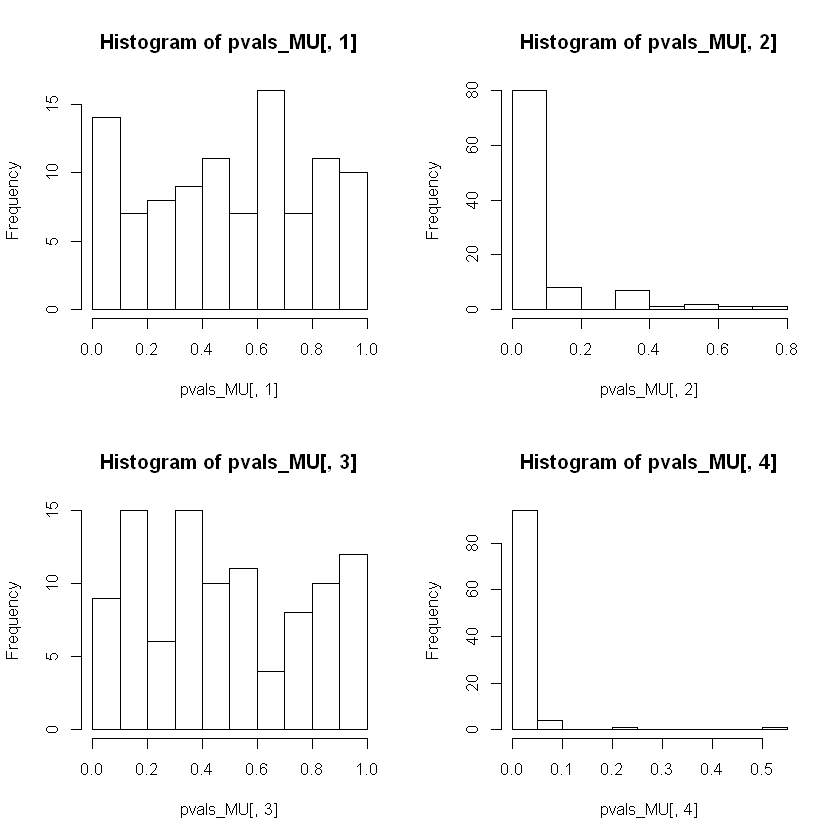
\includegraphics[width=\linewidth]{T_Test_Poisson_YM.png}
	\centering
	\caption{Histograms of p-values obtained from t-tests of the four Poisson networks - Network Autoregressive Model}
	\label{fig: TYM}
\end{figure}
\vspace*{0.5in}
\newpage
\begin{figure}
	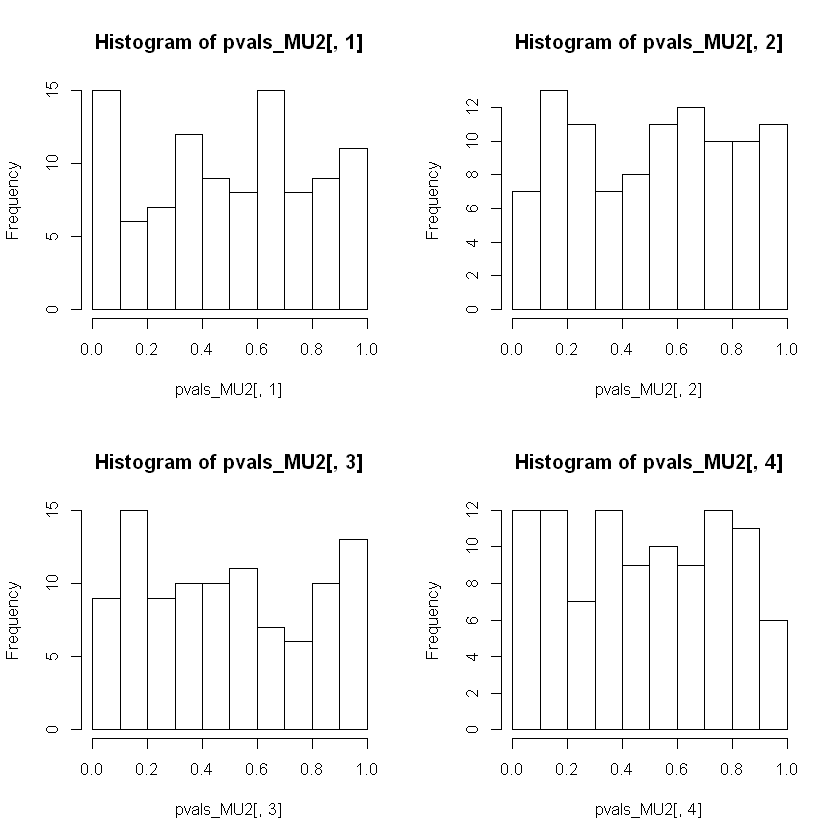
\includegraphics[width=\linewidth]{T_Test_Poisson_YM2.png}
	\centering
	\caption{Histograms of p-values obtained from t-tests of the four Poisson networks - Network Error Autoregressive Model}
	\label{fig: TYM2}
\end{figure}
\vspace*{0.5in}
\newpage
\begin{figure}
	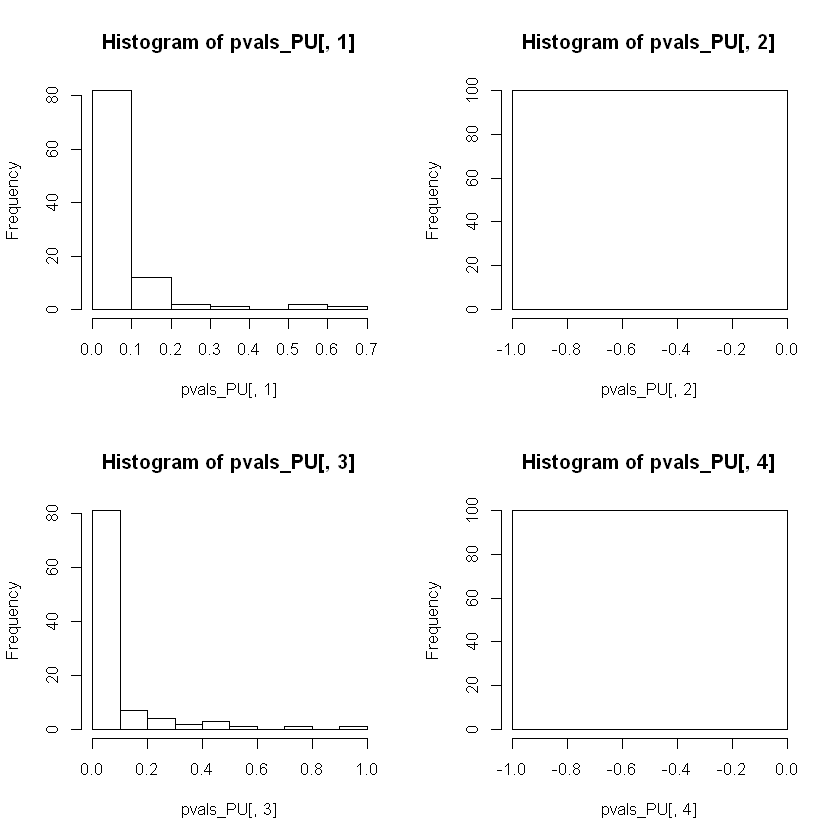
\includegraphics[width=\linewidth]{T_Test_Powerlaw_YP.png}
	\centering
	\caption{Histograms of p-values obtained from t-tests of the powerlaw networks - Network Autoregressive Model}
	\label{fig: TYP}
\end{figure}
\vspace*{0.5in}
\newpage
\begin{figure}
	\includegraphics[width=\linewidth]{T_Test_Powerlaw_YP2.png}
	\centering
	\caption{Histograms of p-values obtained from t-tests of the powerlaw networks - Network Error Autoregressive Model}
	\label{fig: TYP2}
\end{figure}
\begin{figure}
	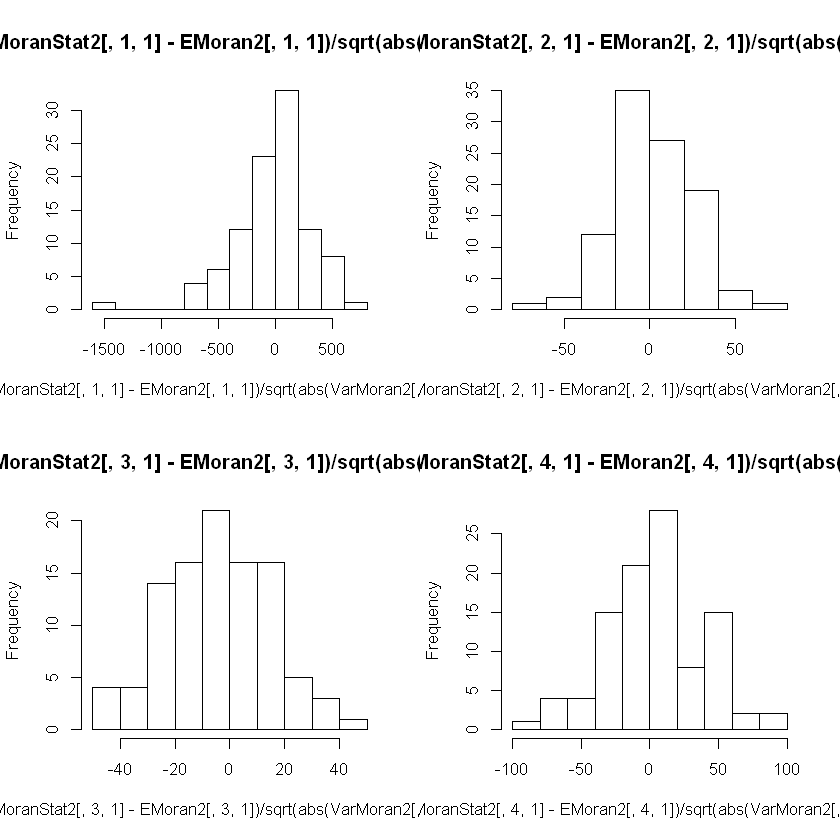
\includegraphics[width=\linewidth]{Moran_Test_Poisson_YM.png}
	\centering
	\caption{Histograms of Moran's I test statistics of the four Poisson networks - Network Autoregressive Model}
	\label{fig: MYM}
\end{figure}
\vspace*{0.5in}
\newpage
\begin{figure}
	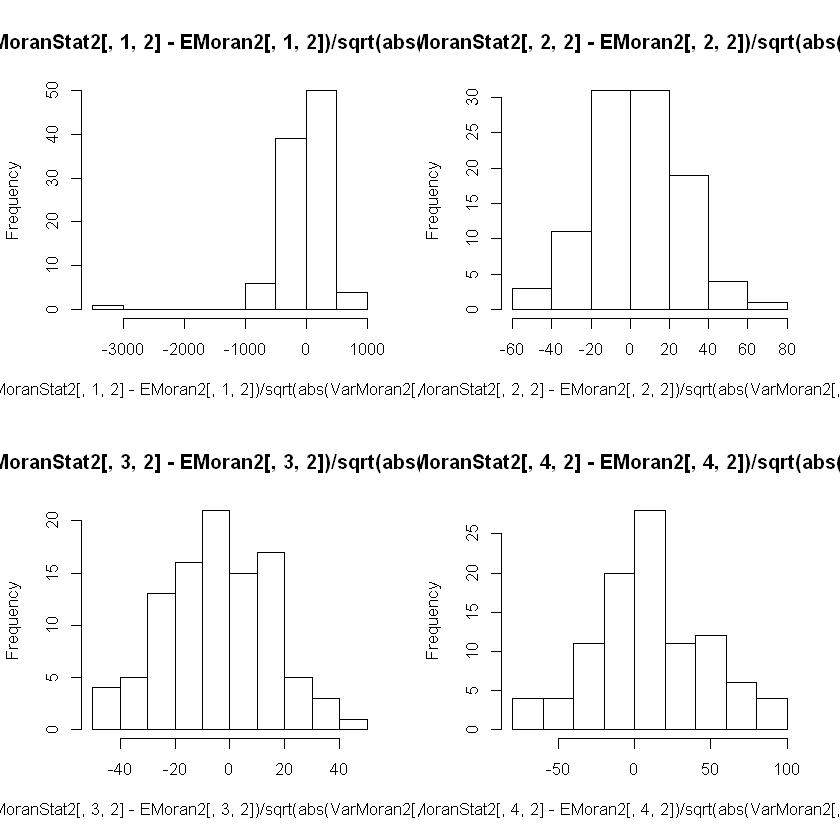
\includegraphics[width=\linewidth]{Moran_Test_Poisson_YM2.png}
	\centering
	\caption{Histograms of Moran's I test statistics of the four Poisson networks - Network Error Autoregressive Model}
	\label{fig: MYM2}
\end{figure}
\vspace*{0.5in}
\newpage
\begin{figure}
	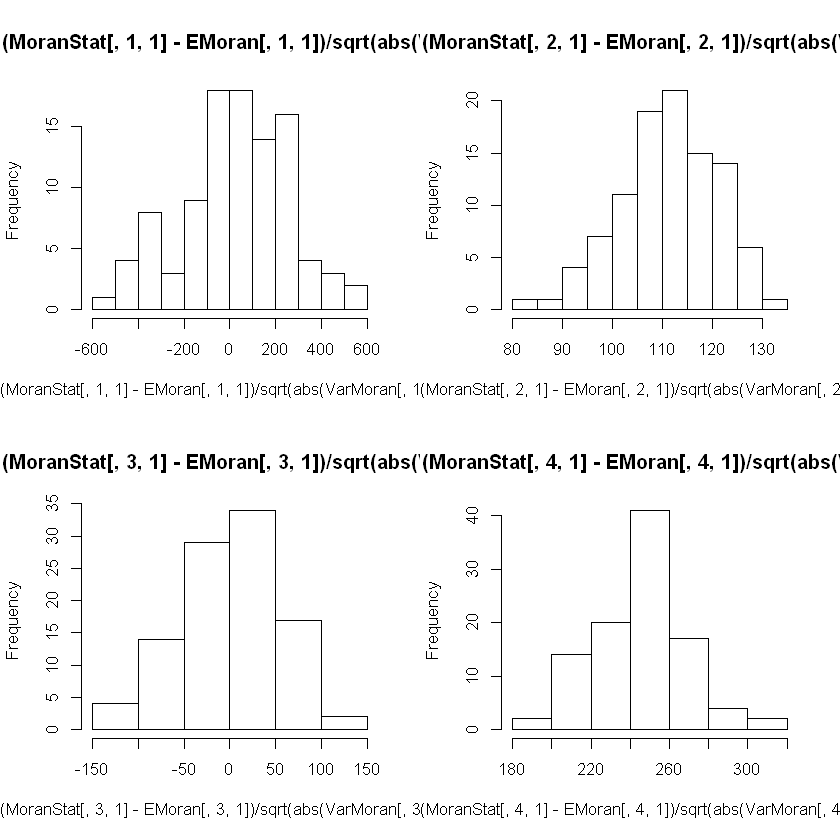
\includegraphics[width=\linewidth]{Moran_Test_Powerlaw_YP.png}
	\centering
	\caption{Histograms of Moran I test statistics of the powerlaw networks - Network Autoregressive Model}
	\label{fig: MYP}
\end{figure}
\vspace*{0.5in}
\newpage
\begin{figure}
	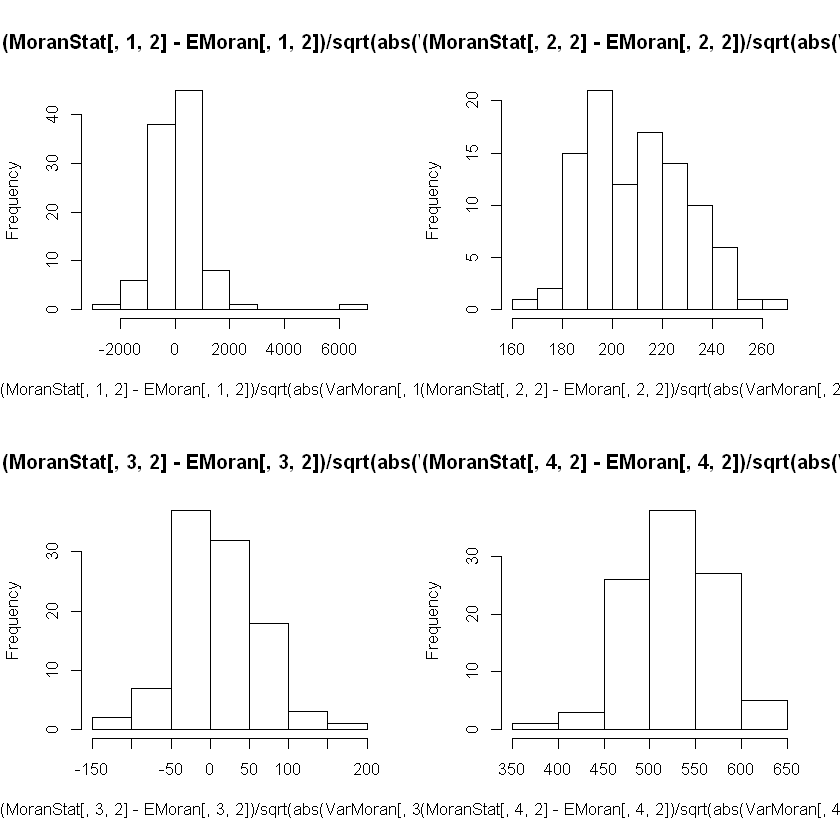
\includegraphics[width=\linewidth]{Moran_Test_Powelaw_YP2.png}
	\centering
	\caption{Histograms of Moran's I test statistics of the powerlaw networks - Network Error Autoregressive Model}
	\label{fig: MYP2}
\end{figure}
\vspace*{0.5in}

The artificial dataset is intended to serve as an intuitive example to illustrate the proposed testing methodologies for different types of networks. In summary, the t-test is effective in screening the networks with Poisson degree distribution and the Moran's I test is more effective for those networks with power-law degree distribution. Given that the degree distributions of most real networks are mixtures of Poisson and power-law distributions, we propose to use the Moran I tests for actual applications.
\newpage
\section{The multi-networks regression model}
Suppose that we have significant networks $G_{1}, G_{2}, \ldots, G_{k}$. Let $A_{1}, A_{2}, \ldots, A_{k}$ be the corresponding row-normalized adjacency matrices respectively. For prediction of the dependent variable $Y$, we consider the network error autoregression model

\begin{equation}
\label{eqn: 7}
Y = X\beta + u,      u \sim n(0, \sigma^{2}KK'),
\end{equation}

\noindent and the network autoregression model

\begin{equation}
\label{eqn: 7a}
Y = KX\beta + u,      u \sim n(0, \sigma^{2}KK'),
\end{equation}

where $K = V^{-1} = \bigg(I_{n} - \sum\limits_{s=1}^{k} \lambda_{s}A_{s}\bigg)^{-1}$, $X=(\mathbbm{1}, X_{1}, \ldots, X_{h})$, and $n = \vert V\vert$. Since $K$ and $V$ are invertible, we require $\vert \sum\limits_{s=1}^{k} \lambda_{s}\vert < 1$. The model parameters are $(\lambda_{1}, \ldots, \lambda_{k}, \beta, \sigma^{2})$. Using the following prior distributions,
\begin{equation}
\label{eqn: 8}
\begin{array}{rl}
\beta &\sim n(\mu_{0}, \Sigma_{0});\\
\\
\sigma^{2} &\sim IG(\alpha_{0},\gamma_{0});\\
\\
\lambda_{s} &\sim \text{Truncated } n\bigg(0,\dfrac{1}{\xi_{s}}\bigg)I\bigg(-1-\sum\limits_{r=1, r \ne s}^{k}\lambda_{r} < \lambda_{s} < 1- \sum\limits_{r=1, r \ne s}^{k}\lambda_{r}\bigg), s=1,2,\ldots,k,
\end{array}
\end{equation}
we derive a Gibbs Sampler of the parameters for the network error autoregression model:
\begin{itemize}
	\item $\beta \vert Y, X, V, \sigma^{2} \sim n\bigg(\mu_{\beta}, \Sigma_{\beta}\bigg),$ where $\Sigma_{\beta}^{-1} = \Sigma_{0}^{-1} + \dfrac{1}{\sigma^{2}}X'V'VX$ and \\ 
	$\mu_{\beta} = \Sigma_{\beta}\bigg(\Sigma_{0}^{-1}\mu_{0} + \dfrac{1}{\sigma^{2}}X'V'VY\bigg)$;
	\item $\sigma^{2} \vert Y, X, V, \beta \sim IG\bigg(\alpha_{0} + \dfrac{n}{2}, \gamma_{0}+\dfrac{1}{2}(Y-X\beta)'V'V(Y-X\beta)\bigg)$;
	\item For $s = 1,2, \ldots, k$, 
	\newline
	\noindent $f(\lambda_{s}\vert Y, X, \beta, \lambda_{r}, r \ne s, \sigma^{2})$
	\begin{equation}
	\label{eqn: 9}
	%\begin{array}{l}
	\begin{aligned}
	% f(\lambda_{s}\vert Y, X, \beta, \lambda_{r}, r \ne s, \sigma^{2}) \\
	& \propto & \big\vert I_{n} - \sum\limits_{r=1}^{k} \lambda_{r}A_{r}\big\vert \exp\bigg\{-\dfrac{1}{2}\bigg[\lambda_{s}^{2}\bigg(\xi_{s} + \dfrac{1}{\sigma^{2}}\text{tr}\big(A_{s}'A_{s}(Y-X\beta)(Y-X\beta)'\big)\bigg)\\
	&& -\dfrac{\lambda_{s}}{\sigma^{2}}\text{tr}\bigg(A_{s}'\bigg(I_{n}-\sum\limits_{r=1, r \ne s}^{k} \lambda_{r}A_{r}\bigg)(Y-X\beta)(Y-X\beta)'\bigg)+\cdots\bigg]\bigg\}\\
	&& \times I\bigg(-1-\sum\limits_{r=1, r \ne s}^{k}\lambda_{r} < \lambda_{s} < 1- \sum\limits_{r=1, r \ne s}^{k}\lambda_{r}\bigg).
	%\end{array}
	\end{aligned}
	\end{equation}
\end{itemize}

and a Gibbs Sampler of the parameters for the network autoregression model:
\begin{itemize}
	\item  $\beta \vert Y, X, V, \sigma^{2} \sim n\bigg(\mu_{\beta}, \Sigma_{\beta}\bigg),$ where $\Sigma_{\beta}^{-1} = \Sigma_{0}^{-1} + \dfrac{1}{\sigma^{2}}X'X$ and \\ 
	$\mu_{\beta} = \Sigma_{\beta}\bigg(\Sigma_{0}^{-1}\mu_{0} + \dfrac{1}{\sigma^{2}}X'VY\bigg)$;
	\item $\sigma^{2} \vert Y, X, V, \beta \sim IG\bigg(\alpha_{0} + \dfrac{n}{2}, \gamma_{0}+\dfrac{1}{2}(VY-X\beta)'(VY-X\beta)\bigg)$;
	\item For $s = 1,2, \ldots, k$, 
	\newline
	\noindent $f(\lambda_{s}\vert Y, X, \beta, \lambda_{r}, r \ne s, \sigma^{2})$
	\begin{equation}
	\label{eqn: 9a}
	%\begin{array}{l}
	\begin{aligned}
	% f(\lambda_{s}\vert Y, X, \beta, \lambda_{r}, r \ne s, \sigma^{2}) \\
	& \propto & \big\vert I_{n} - \sum\limits_{r=1}^{k} \lambda_{r}A_{r}\big\vert \exp\bigg\{-\dfrac{1}{2}\bigg[\lambda_{s}^{2}\bigg(\xi_{s} + \dfrac{1}{\sigma^{2}}Y'A_{s}'A_{s}Y\bigg)\\
	&& -\dfrac{\lambda_{s}}{\sigma^{2}}Y'A_{s}'\bigg(\bigg(I_{n}-\sum\limits_{r=1, r \ne s}^{k} \lambda_{r}A_{r}\bigg)Y-X\beta\bigg)-\cdots\bigg]\bigg\}\\
	&& \times I\bigg(-1-\sum\limits_{r=1, r \ne s}^{k}\lambda_{r} < \lambda_{s} < 1- \sum\limits_{r=1, r \ne s}^{k}\lambda_{r}\bigg).
	%\end{array}
	\end{aligned}
	\end{equation}
\end{itemize}
	The MH algorithm is applied to generate the random numbers from the conditional distribution in (\ref{eqn: 9}). Let 
	\[
	f_{V} = n\big(\mu_{\lambda_{s}}, \Sigma_{\lambda_{s}}\big)I\bigg(-1-\sum\limits_{r=1, r \ne s}^{k}\lambda_{r} < \lambda_{s} < 1- \sum\limits_{r=1, r \ne s}^{k}\lambda_{r}\bigg),
	\]
	where 
	\[
	\Sigma_{\lambda_{s}}^{-1} = \xi_{s} + \dfrac{1}{\sigma^{2}}\text{tr}\big(A_{s}'A_{s}(Y-X\beta)(Y-X\beta)'\big)
	\]
	and 
	\[
	\mu_{\lambda_{s}} = \dfrac{\Sigma_{\lambda_{s}}}{\sigma^{2}}\text{tr}\bigg(A_{s}'\bigg(I_{n}-\sum\limits_{r=1, r \ne s}^{k} \lambda_{r}A_{r}\bigg)(Y-X\beta)(Y-X\beta)'\bigg).
	\]
	
	\noindent The MH algorithm is applied to generate the random numbers from the conditional distribution in (\ref{eqn: 9a}). Let 
	\[
	f_{V} = n\big(\mu_{\lambda_{s}}, \Sigma_{\lambda_{s}}\big)I\bigg(-1-\sum\limits_{r=1, r \ne s}^{k}\lambda_{r} < \lambda_{s} < 1- \sum\limits_{r=1, r \ne s}^{k}\lambda_{r}\bigg),
	\]
	where 
	\[
	\Sigma_{\lambda_{s}}^{-1} = \xi_{s} + \dfrac{Y'A_{s}A_{s}Y}{\sigma^{2}}
	\]
	and 
	\[
	\mu_{\lambda_{s}} = \dfrac{\Sigma_{\lambda_{s}}}{\sigma^{2}}Y'A_{s}'\bigg(\bigg(I_{n}-\sum\limits_{r=1, r \ne s}^{k} \lambda_{r}A_{r}\bigg)Y - X\beta\bigg).
	\]
	
	\noindent To generate $\lambda_{s} \sim f(\lambda_{s} \vert Y, \cdot)$, we first generate $v$ from $f_{V}$ and set $Z_{0} = v$. Then, the following steps are iterated for $i=1,2,\ldots$ :
	\begin{itemize}
		\item Generate $u_{i} \sim U(0,1)$, $v_{i} \sim f_{V}$ and calculate
		\[
		\phi_{i} = \min\bigg\{\dfrac{\bigg\vert I_{n} - v_{i}A_{s} - \sum\limits_{r=1, r \ne s}\lambda_{r}A_{r}\bigg\vert}{\bigg\vert I_{n} - Z_{i-1}A_{s} - \sum\limits_{r=1, r \ne s}\lambda_{r}A_{r}\bigg\vert},1\bigg\};
		\]
		\item Set $Z_{i} = \begin{cases} v_{i} & \text{if }u_{i} \le \phi_{i}\\ Z_{i-1} & \text{if }u_{i} > \phi_{i}.\end{cases}$ As $i \rightarrow \infty$, $Z_{i}$ converges in distribution to $\lambda_{s}$.
	\end{itemize}

For practical purposes, we initialize the Gibbs Sampler with the following random number generations:
\begin{itemize}
	\item $\beta_{1}$ is generated from $n(\mu_{0}, \Sigma_{0})$.
	\item $\sigma_{1}^{2}$ is generated from $IG(\alpha_{0}, \gamma_{0})$.
	\item For $\lambda$, we start with the following random number generations:
	\[
	\begin{array}{rl}
	\lambda_{1,1} &\sim n\bigg(0,\dfrac{1}{\xi_{1}}\bigg)I(-1 < \lambda_{1,1} < 1),\\
	\lambda_{2,1} &\sim n\bigg(0,\dfrac{1}{\xi_{2}}\bigg)I(-1-\lambda_{1,1} < \lambda_{2,1} < 1-\lambda_{1,1}),\\
	&\ldots\\ 
	\lambda_{k,1} &\sim n\bigg(0,\dfrac{1}{\xi_{k}}\bigg)I(-1-\sum\limits_{r=1}^{k-1}\lambda_{r,1} < \lambda_{k,1} < 1-\sum\limits_{r=1}^{k-1}\lambda_{r,1}).
	\end{array}
	\]
	Then, the following steps are iterated for $j = 1,2,\ldots,k$,
	\[
	\lambda_{j,1} \sim n\bigg(0,\dfrac{1}{\xi_{j}}\bigg)I(-1-\sum\limits_{r=1, r \ne j}^{k}\lambda_{r,1} < \lambda_{j,1} < 1-\sum\limits_{r=1, r \ne k}^{k}\lambda_{r,1}).
	\]
\end{itemize}
Given the first set of random numbers, these iteration steps in our Gibbs Sampler can be applied to find random numbers from the joint posterior distribution of the model parameters.
\newline

For a prediction on the new data $(Y_{*},X_{*})$, we have the distribution
\[
\begin{bmatrix} u_{*}\\u\end{bmatrix} \sim n\Bigg(0, \sigma^{2}\begin{bmatrix} U_{*,*} & U_{*,t}\\ U_{*,t}' & U_{t,t}\end{bmatrix}\Bigg),
\]
where $U = KK' = \begin{bmatrix} U_{*,*} & U_{*,t}\\ U_{*,t}' & U_{t,t}\end{bmatrix}$, and the index $t$ corresponds to the original training data. The multivariate normal theory implies that
\[
u_{*} \big\vert u, K \sim n\big(U_{*,t}U_{t,t}^{-1}u, U_{*,*} - U_{*,t}U_{t,t}^{-1}U_{*,t}'\big).
\]
Thus, for the network error autoregressive model, the prediction distribution of $Y_{*}$ conditioned on $X_{*}, X, Y, K, \beta$, and $\sigma^{2}$ is
\[
Y_{*} \big\vert X_{*}, X, Y, K, \beta, \sigma^{2} \sim n\bigg(X_{*}\beta + U_{*,t}U_{t,t}^{-1}(Y-X\beta), U_{*,*} - U_{*,t}U_{t,t}^{-1}U_{*,t}'\bigg).
\]
$Y_{*}$ can be predicted with 
\begin{equation}
\label{eqn: 14}
\hat{Y_{*}} = X_{*}\hat{\beta} + U_{*,t}(\hat{\lambda})V_{t,t}(\hat{\lambda})^{-1}(Y-X\hat{\beta}).
\end{equation}

\noindent and, for the network autoregressive model, the prediction distribution of $Y_{*}$ conditioned on $X_{*}, X, Y, K, \beta$, and $\sigma^{2}$ is
\[
Y_{*} \big\vert X_{*}, X, Y, K, \beta, \sigma^{2} \sim n\bigg(KX_{*}\beta + U_{*,t}U_{t,t}^{-1}(Y-KX\beta), U_{*,*} - U_{*,t}U_{t,t}^{-1}U_{*,t}'\bigg).
\]
$Y_{*}$ can be predicted with 
\begin{equation}
\label{eqn: 14}
\hat{Y_{*}} = KX_{*}\hat{\beta} + U_{*,t}(\hat{\lambda})V_{t,t}(\hat{\lambda})^{-1}(Y-KX\hat{\beta}).
\end{equation}
%Using the simulated $Y$ in section 2, figure 8 displays the histogram of $\hat{\rho}$. The histogram in the left hand side uses $W_{1}$ and that in the right hand side uses $W_{3}$. We see that the distribution of $\hat{\rho}$ for the Poisson networks is more scatter and that for the power-law networks is more concentrated. As indicated in Zhou, et al. (2015), the distributions of $\hat{\rho}$ are asymptotically normal in both cases, despite the marked difference. We will apply the single-network regression model to two data sets in section 5. 
%\begin{figure}
%  \includegraphics[width=\linewidth]{estimated_rhos2.png}
%  \caption{Histogram of estimated $\rho$}
%  \label{fig: estimated_rhos}
%\end{figure}

\section{Simulation Studies}
We generate 8 networks, 4 of them have Poisson degree distributions (with probability of attachments 0.2, 0.25, 0.28 and 0.3, respectively) and 4 of them have power-law degree distributions (with degree exponents 2, 2.1, 2.17 and 2.5). The 8 networks are mixed to create 4 networks $G_{1}$, $G_{2}$, $G_{3}$ and $G_{4}$, respectively. Each network $G_{i}$ is a mixture of a Poisson degree distributed network and a power-law degree distributed network. The mixing proportions are $30\%$ Poisson network and $70\%$ power-law network. The exponent of the degree distributions of the mixed networks are 22.81, 23.02, 21.78 and 21.88 respectively. All the mixed networks are row-normalized. Using a randomly generated matrix of explanatory variables, with $n=2000$ number of observations and $p=5$ number of predictors, and the parameters $\beta = (0.1,-0.2,0.4,-0.1,0.25,0.15)$, $\lambda = (0.2,0.2,0.2,0.2)$, $w = (0.25,-0.25,0.25,0.25)$, and $\sigma^{2}=1.0$,  we generate 100 responses using the error autoregression model (\ref{eqn: 7}), where $Y = X\beta + \bigg(I_{n}-\sum\limits_{i=1}^{4}\lambda_{i}G_{i}\bigg)^{-1}\varepsilon$, and 100 responses using the network autoregression model (\ref{eqn: 7a}), where $Y = \bigg(I_{n}-\sum\limits_{i=1}^{4}w_{i}G_{i}\bigg)^{-1}(X\beta + \varepsilon)$. The $\varepsilon$ is a random vector from the normal distribution with mean $(0,0,\ldots,0)$ and variance $\sigma^{2}I_{n}$. For each response, we randomly select $80\%$ of the observations to estimate the parameters of the corresponding model using the Gibbs Samplers developed in section 4. The posterior distributions of the parameters of the two models are listed in Table \ref{table1c} and Table \ref{table1d} respectively. A typical prediction of the responses on the testing data (the remaining $20\%$ of the observations) is presented in Figure \ref{fig: Pred}.

\begin{table}
	\centering
	\caption{Descriptive statistics of the posterior distributions of the error autoregression model}
	\label{table1c}
	\begin{tabular}{|c|c|c|c|c|c|}
		\hline
		Parameter & Mean & Median & Standard Deviation & Skewness & Kurtosis\\
		\hline
		$\lambda_{1}$ & 0.1954 & 0.1946 & 0.045 & 0.4307 & 2.8346\\
		\hline
		$\lambda_{2}$ & 0.2219 & 0.2235 & 0.042 & -0.1043 & 3.0625\\
		\hline
		$\lambda_{3}$ & 0.2146 & 0.2139 & 0.048 & 0.4345 & 2.8560\\
		\hline
		$\lambda_{4}$ & 0.1847 & 0.1855 & 0.0435 & -0.1792 & 2.787\\
		\hline
		$\beta_{0}$ & 0.09696 & 0.0972 & 0.0667 & -0.1436 & 3.0983\\
		\hline
		$\beta_{1}$ & -0.1994 & -0.1994 & 0.000497 & 0.1607 & 2.8397\\
		\hline
		$\beta_{2}$ & 0.4003 & 0.4003 & 0.000493 & -0.14642 & 2.7983\\
		\hline
		$\beta_{3}$ & -0.09975 & -0.09978 & 0.00054 & 0.1103 & 2.8109\\
		\hline
		$\beta_{4}$ & 0.2494 & 0.2495 & 0.000490 & -0.4200 & 3.1720\\
		\hline
		$\beta_{5}$ & 0.14980 & 0.14979 & 0.000504 & 0.13448 & 3.0834\\
		\hline
		$\sigma^{2}$ & 0.8550 & 0.84010 & 0.31440 & 0.2130 & 3.4662\\
		\hline
	\end{tabular}
\end{table}

\begin{table}
	\centering
	\caption{Descriptive statistics of the posterior distributions of the network autoregression model}
	\label{table1d}
	\begin{tabular}{|c|c|c|c|c|c|}
		\hline
		Parameter & Mean & Median & Standard Deviation & Skewness & Kurtosis\\
		\hline
		$w_{1}$ & 0.2434 & 0.2373 & 0.0952 & 0.1561 & 2.8754\\
		\hline
		$w_{2}$ &-0.2682 & -0.2662 & 0.0361 & -0.2060 & 3.3430\\
		\hline
		$w_{3}$ & 0.2477 & 0.2499 & 0.04364 & -0.1672 & 3.0250\\
		\hline
		$w_{4}$ & 0.2398 & 0.2406 & 0.01998 & -0.1753 & 3.3436\\
		\hline
		$\beta_{0}$ & 0.08254 & 0.08264 & 0.01524 & 0.1199 & 3.5711\\
		\hline
		$\beta_{1}$ & -0.1900 & -0.1895 & 0.00231 & -0.1680 & 3.1192\\
		\hline
		$\beta_{2}$ & 0.3817 & 0.3812 & 0.00217 & -0.1900 & 2.9395\\
		\hline
		$\beta_{3}$ & -0.0996 & -0.0997 & 0.00217 & -0.1785 & 2.8609\\
		\hline
		$\beta_{4}$ & 0.2683 & 0.2679 & 0.002398 & 0.2235 & 2.7668\\
		\hline
		$\beta_{5}$ & 0.1469 & 0.1468 & 0.00254 & 0.1475 & 3.4919\\
		\hline
		$\sigma^{2}$ & 1.1093 & 1.095 & 0.4267 & 0.1577 & 3.5852\\
		\hline
	\end{tabular}
\end{table}

\begin{figure}
	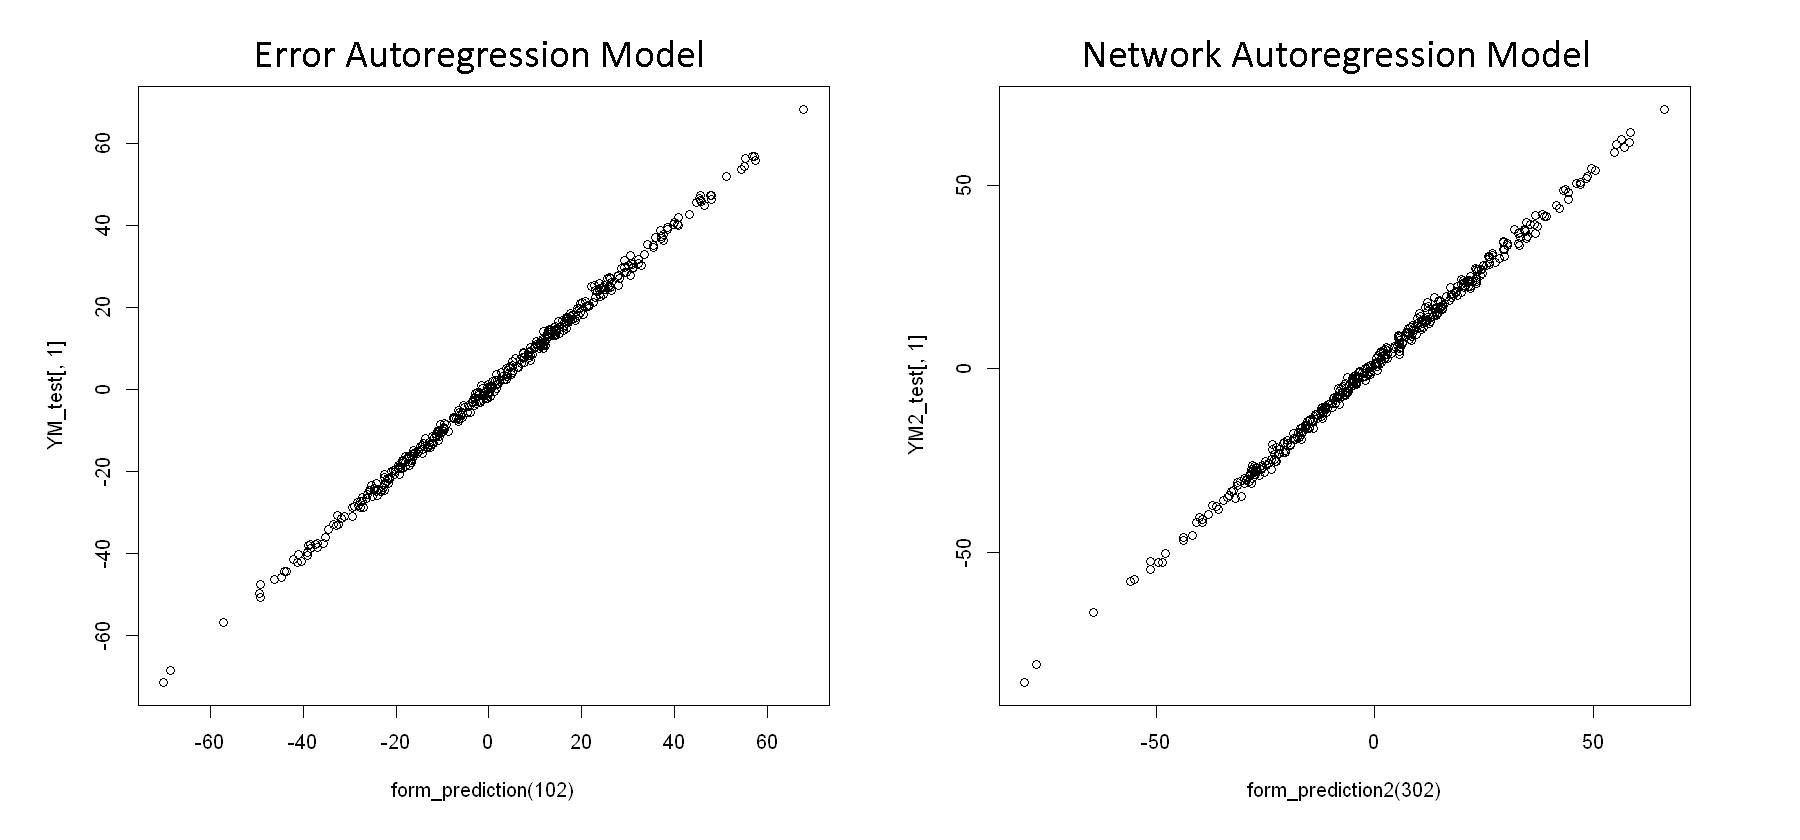
\includegraphics[width=\linewidth]{prediction_simulations.png}
	\centering
	\caption{A typical prediction of the responses on the testing data}
	\label{fig: Pred}
\end{figure}
	

\section{Applications to real data}
\subsection{The North Carolina Sudden Infant Deaths}
This section uses a dataset available in the R-package spdep (\cite{R20}) to demonstrate the multiple network regression model. The dataset contains the number of live births (BIR), non-white live births (NWBIR) and sudden infant deaths (SID) from July 1, 1974 to June 30, 1978 and from July 1, 1979 to June 30, 1984 in 100 counties of North Carolina, USA. Figure \ref{fig: nc_SID79} displays the SIDS79 in a color gradient. From the figure, adjacent regions have related numbers of sudden infant deaths. Figure \ref{fig: SID79} reveals that SID79 is linearly related with SID74 and is quadratically related with $\log(\text{BIR79})$ or $\log(\text{BIR74})$. Because many regions have zero sudden infant death, an indicator variable named zeroind is created to isolate these regions. The objective is to develop a network regression model which predicts SID79. The explanatory variables are $\log(\text{BIR79})$, $\log(\text{BIR79})^{2}$, SID74, $\log(\text{BIR74})$, $\log(\text{BIR74})^{2}$ and zeroind. Using the shapefile of North Carolina regions, three weight matrices containing contiguity relations or function of distances are created.
\begin{itemize}
	\item \textbf{Nearest-neighbor weight matrix:} \\
	For each region, five regions with the smallest centoid distances are chosen as neighbors. 
	\item \textbf{Spatial contiguity weight matrix:} \\
	Two regions are neighbor if they have common boundary. That is, let $\partial \{i\}$ be the boundary of the region $i$. Region $i$ and region $j$ are neighbor if $\partial \{i\} \cup \partial \{j\} \ne \O$.
	\item \textbf{Share bounary weight matrix:} \\
	Let $\ell_{i,j}$ be the length of $\partial \{i\} \cup \partial \{j\}$ and $d_{i,j}$ be the centroid distance between region $i$ and region $j$. The spatial weight between region $i$ and region $j$ is $w_{i,j} = \dfrac{\ell_{i,j}d_{i,j}^{-1}}{\sum\limits_{k \ne i} \ell_{i,k}d_{i,k}^{-1}}$.
\end{itemize}
All three weight matrices are row-normalized. For each matrix, we perform the Moran's I normality test as described in section 3. The p-values obtained from the test are reported in table \ref{table1}. The nearest-neighbor weight matrix is the most significant, followed by the share-boundary weight matrix. These two networks are chosen to be the candidate networks for our error autoregression model. Next, the regions are split into training and testing sets, in which 75 regions are assigned for training, and the remaining 25 regions for testing. Using the training set, the Gibbs Sampler developed in Section 4 is applied to generate random numbers from the joint posterior distribution of the model parameters $(\lambda_{1}, \lambda_{2}, \beta, \sigma^{2})$. Table \ref{table2} presents the summary statistics of the posterior distributions of $(\lambda_{1}, \lambda_{2}, \beta, \sigma^{2})$. For each set of the model parameters $(\lambda_{1}, \lambda_{2}, \beta, \sigma^{2})$, we predict SID79 with the testing data using (\ref{eqn: 14}). The mean square root of prediction errors is $3.5822$. The actual and mean predicted SID79 in the testing data are presented in Figure \ref{fig: predicted_SID79}. As shown in the figure, the multi-network error autoregression model predicts the dependent variable SID79 in the testing data reasonably well.
\begin{table}
	\centering
	\caption{p-values for the significance testing of the weight matrices}
	\label{table1}
	\begin{tabular}{|c|c|c|c|}
		\hline
		\multirow{ 2}{*}{Network Test} & Nearest-neighbor & Spatial Contiguity & Share Boundary\\
		& Weight Matrix & Weight Matrix & Weight Matrix\\
		\hline
		Moran I test & 0.00084 & 0.25943 & 0.01177\\
		\hline
	\end{tabular}
\end{table}

\begin{table}
	\centering
	\caption{Descriptive statistics of the posterior distributions}
	\label{table2}
	\begin{tabular}{|c|c|c|c|c|c|}
		\hline
		Parameter & Mean & Median & Standard Deviation & Skewness & Kurtosis\\
		\hline
		$\lambda_{1}$ & -0.16635 & -0.16635 & 0.00006 & -0.14541 & 2.8408\\
		\hline
		$\lambda_{2}$ & -0.53720 & -0.53722 & 0.0002 & 0.41077 & 2.54746\\
		\hline
		$\beta_{0}$ & 130.7466 & 130.7468 & 0.00966 & -0.19583 & 3.97191\\
		\hline
		$\beta_{1}$ & 29.15357 & 29.15333 & 0.001743 & -0.06266 & 3.0527\\
		\hline
		$\beta_{2}$ & -2.18407 & -2.18406 & 0.0012 & 0.03523 & 3.0623\\
		\hline
		$\beta_{3}$ & 0.25439 & 0.25439 & 0.00005 & -0.08483 & 3.045\\
		\hline
		$\beta_{4}$ & -69.330 & -69.330 & 0.018134 & 0.0494 & 3.08117\\
		\hline
		$\beta_{5}$ & 5.2970 & 5.2970 & 0.001309 & -0.003054 & 3.081\\
		\hline
		$\beta_{6}$ & -3.32070 & -3.32072 & 0.00075 & 0.3599 & 2.4488\\
		\hline
		$\sigma^{2}$ & 0.0000022 & 0.0000022 & 0.000000072 & 0.3973 & 2.4262\\
		\hline
	\end{tabular}
\end{table}

\begin{figure}
	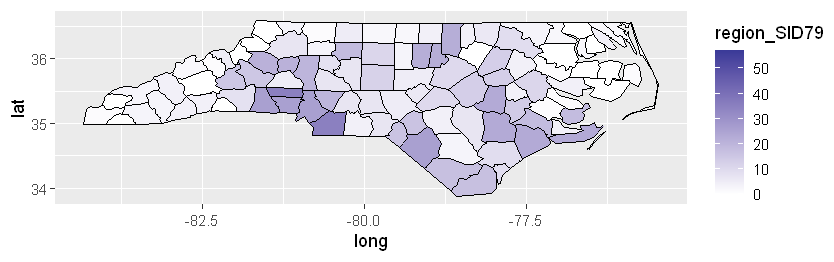
\includegraphics[width=\linewidth]{regions_SID79.png}
	\centering
	\caption{Sudden Infant Deaths between July 1, 79 and June 30, 84 of NC}
	\label{fig: nc_SID79}
\end{figure}

\begin{figure}
	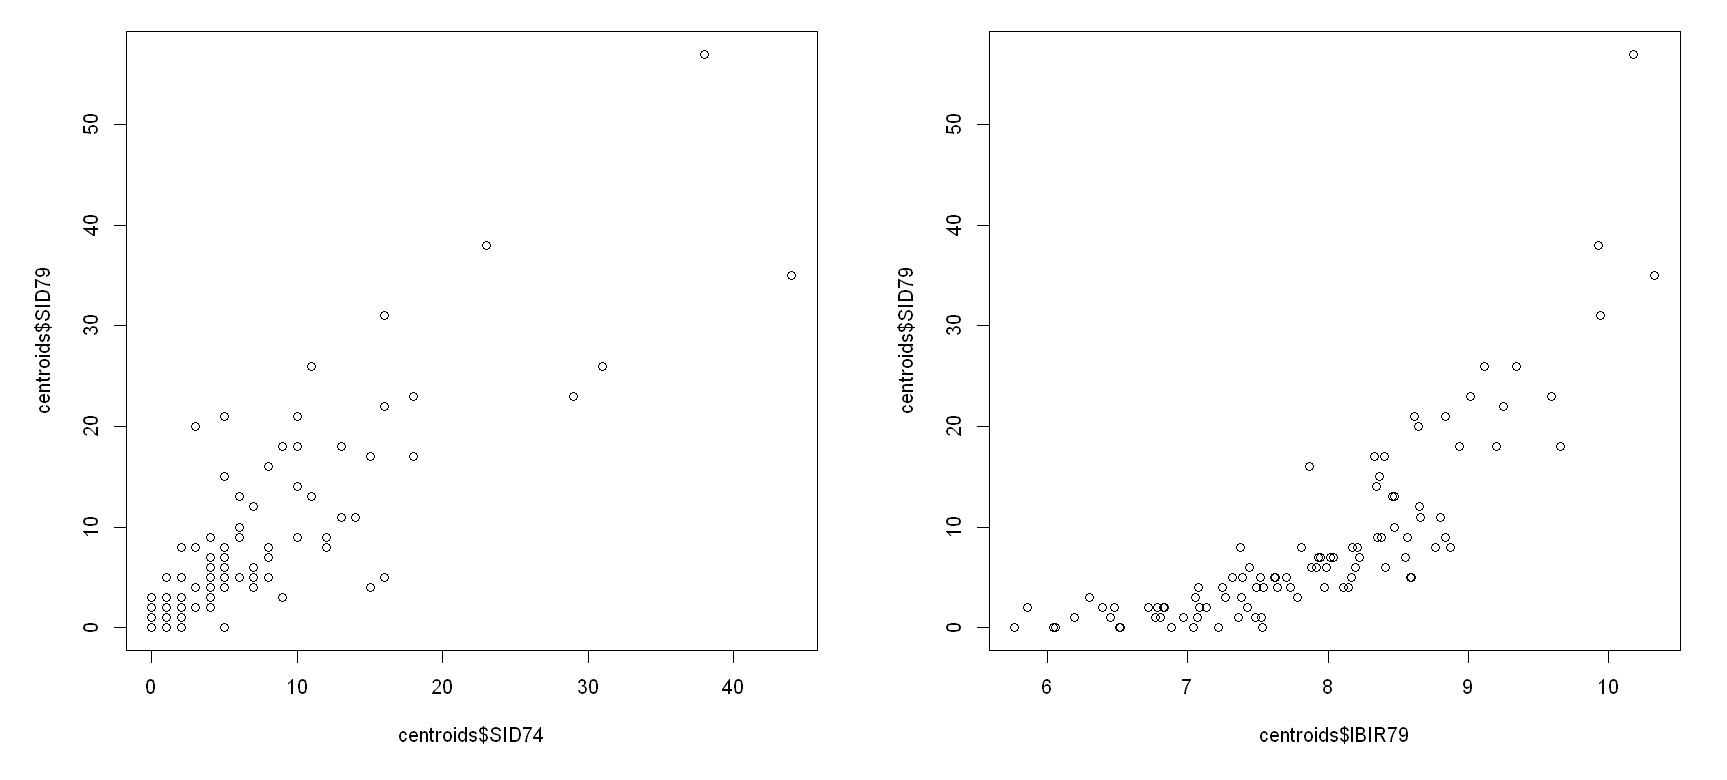
\includegraphics[width=\linewidth]{SID79_n_X.png}
	\caption{SID79 vs SID74 (left) and SID79 vs log(BIR79) (right)}
	\label{fig: SID79}
\end{figure}

\begin{figure}
	\centering
	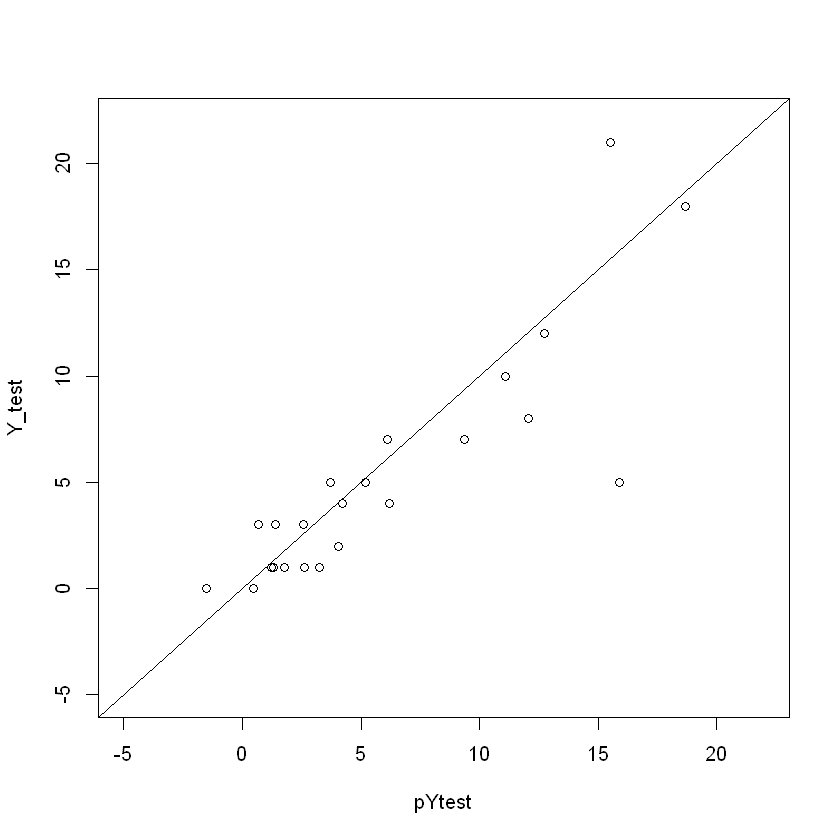
\includegraphics[width=60mm]{pred_test_NC_SID79_2.png}
	\caption{Actual vs Mean predicted SID79 on the testing data}
	\label{fig: predicted_SID79}
\end{figure}

\subsection{Predicting the changes in Stock Prices}
The second dataset consists of (i) the changes in stock prices between the first trading day of 2018 and that of 2019, and (ii) the changes in a set of 21 company attributes in the same period for 555 listed companies in the Hong Kong stock exchange. The company attributes are volume, current ratio, quick ratio, long term debt to equity, total debt to equity, debt to capital, return on equity, return on capital, return on total assets, operating profit margin, net profit margin, inventory turnover, dividend payout, net profit, net profit growth, earning per share, earning per share growth, dividend per share, price per earning, yield and net asset value. The relationships between changes in company attributes and changes in stock prices are illustrated in Figure \ref{fig:prices}. We define the dependent variable $Y$ as the change in stock prices. The data matrix $X$ is constructed in the usual way such that the first column is ones and subsequent columns are the company attributes. 
\newline

In addition to individual company attributes, two companies may be related in many ways. For instances, they may share a major shareholder, a common member in their board of directors or a related company such as a customer, a supplier and/or a parent company. Their business strategies are likely influenced by their common membership(s). The common members might influence their companies in the following ways. Firstly, when two companies have the same parent company, the financial health of their parent company could impact their own business interests. Secondly, the common directors could provide a set of skills beneficial to both companies. Thirdly, the business strategy of their common customer(s) could affect their profitability. Part of such influences can be captured by creating a network of relations for each definition of neighbors. Two companies are neighbor when they have a common major shareholder, a common member in their board of directors or a common related company. In addition, the company business usually belongs to one of the many industrial groups and a company can have businesses in multiple industries. When two companies have businesses in the same industrial group, their stock prices are likely moved in concordant possibly with different degrees. An industry network can be defined in which two companies are linked if they have business in the same industrial group. Finally, the conditional dependent structure among the stock prices of the companies also forms a network. 
\newline

The following information was collected for each company, including the types of industry $WI$, the auditors $WA$, the solicitors $WS$, the company secretaries $WC$, the company executives $WE$ and the shareholders $WSH$. For each of these variables, a network was defined such that an edge between a company pair is formed when they share the same level in the variable. Apart from these six networks, we collected daily close prices between Jan 2014 and Jan 2018 for each company. The partial correlations of the close prices for every pair of the companies in the dataset are then computed. Two companies are connected by an edge if their partial correlation is larger than a fixed threshold. Clearly, the size of this threshold determines the number of edges in the partial correlation network. The threshold is set at 0.15 so that the number of edges in the network is about double the number of nodes. 
\newline

Let $A$ be the adjacency matrix of a network. $A^{\ell}$, where $\ell$ is an integer, is a matrix whose $(i,j)$ element is the number of paths of length $\ell$ connecting node $i$ and node $j$. For a given value of $\alpha \in (0,1)$, we can consider the matrix
\begin{equation}
\label{eqn: 15}
\begin{array}{rl}
GA &= A + \alpha A^{2} + \alpha^{2} A^{3} + \cdots\\
&= A(I_{n} + \alpha A + \alpha^{2} A^{2} + \cdots )\\ 
&= A(I_{n} - \alpha A)^{-1}.
\end{array}
\end{equation}
$GA$ is a matrix whose $(i,j)$ element is the direct sum of the collection of all paths connecting node $i$ and node $j$, exponentially damped by the length to give the shorter paths with more weights. Being an $\infty$th graph power of $A$, $GA$ can be regarded as its boosted version. 
\newline

Except for the partial correlation network, we computed the boosted version for each of the six networks with $\alpha = 0.75$. They are labelled as $GWI$, $GWA$, $GWS$, $GWC$, $GWE$, and $GWSH$. All six adjacency matrices, along with their boosted version, are row-normalized. The Moran's I test is applied to each of these matrices. The corresponding p-values are reported in Table \ref{table3}, which indicates that the networks $W$, $GWA$, $GWS$, $GWC$, $GWE$, and $GWSH$ are significant. As in the previous example, we split the listed companies into training and testing sets with $80\%$ used for training and remaining $20\%$ for testing. Using the training set, the Gibbs Samplers developed in Section 3 are applied to generate random numbers from the joint posterior distribution of the model parameters $(\lambda_{1}, \lambda_{2}, \lambda_{3}, \lambda_{4}, \lambda_{5}, \lambda_{6}, \beta, \sigma^{2})$ for the error autoregression model and $(w_{1}, w_{2}, w_{3}, w_{4}, w_{5}, w_{6}, \beta, \sigma^{2})$ for the network autoregression model. Table \ref{table4} presents the summary statistics of the posterior distributions of $(\lambda_{1}, \lambda_{2}, \lambda_{3}, \lambda_{4}, \lambda_{5}, \lambda_{6}, \beta, \sigma^{2})$ for the error autoregression model and Table \ref{table4a} presents the summary statistics of the posterior distributions of $(w_{1}, w_{2}, w_{3}, w_{4}, w_{5}, w_{6}, \beta, \sigma^{2})$ for the network autoregression model. The significance explanatory variables that affect $Y$ are Volume, Long Term Debt to Equity Ratio, Total Debt to Equity, Return on Capital and NAV. 

For each set of the model parameters $(\lambda_{1}, \lambda_{2}, \lambda_{3}, \lambda_{4}, \lambda_{5}, \lambda_{6}, \beta, \sigma^{2})$ for the error autoregression model and $(w_{1}, w_{2}, w_{3}, w_{4}, w_{5}, w_{6}, \beta, \sigma^{2})$ for the network autoregression model, we predict the change in stock prices with the testing data using (\ref{eqn: 14}), respectively. The mean square root of the prediction errors is $9.95$ for the error autoregression model and $21.63$ for the network autoregression model. The actual and mean predicted change in stock prices in the testing data are presented in Figure \ref{fig: predicted_stocks}. As shown in the figure, the multiple network regression model predicts the dependent variable in the testing data reasonably well.

\begin{figure}
	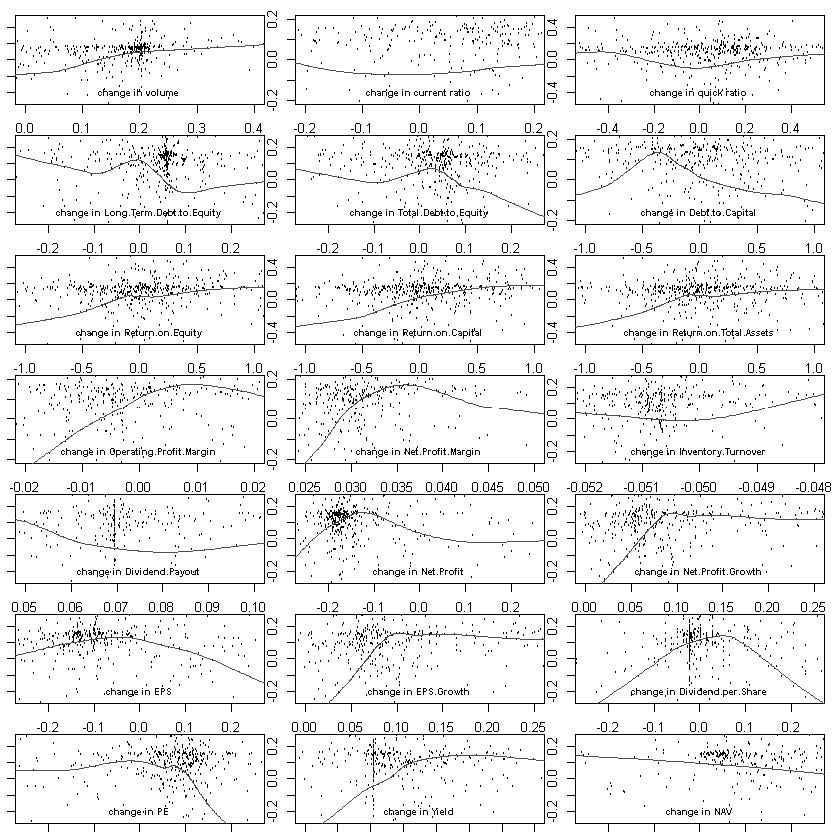
\includegraphics[width=\linewidth]{ps.jpg}
	\caption{Changes in company attributes vs Change in prices}
	\label{fig:prices}
\end{figure}

\begin{table}
	\centering
	\caption{p-values for testing the significance of the network matrices}
	\label{table3}
	\begin{tabular}{|c|c|c|c|c|c|c|c|}
		\hline
		 & W & WI & WA & WS & WC & WE & WSH\\
		\hline
		Moran I test & 0.00916 & 0.3674 & 0.5938 & 0.4571 & 0.7142 & 0.3121 & 0.9648\\
		\hline
		\hline
		 &  & GWI & GWA & GWS & GWC & GWE & GWSH\\
		\hline
		Moran I test &  & 0.6552 & 0.0 & 0.0025 & 0.0072 & 0.015 & 0.096\\
		\hline
	\end{tabular}
\end{table}

\begin{table}
	\small
	\centering
	\caption{Descriptive statistics of the posterior distributions of the error autoregression model}
	\label{table4}
	\begin{tabular}{|c|c|c|c|c|c|}
		\hline
		Parameter & Mean & Median & Standard Deviation & Skewness & Kurtosis\\
		\hline
		$\lambda_{1}$ & 0.2774 & 0.2690 & 0.0574 & 0.6133 & 3.8054\\
		\hline
		$\lambda_{2}$ & -0.2919 & -0.2766 & 0.1065 & -0.1331 & 2.9656\\
		\hline
		$\lambda_{3}$ & 1.3181 & 1.2672 & 0.4293 & 0.6041 & 3.6231\\
		\hline
		$\lambda_{4}$ & -1.780 & -1.7562 & 0.2596 & -0.6701 & 3.5354\\
		\hline
		$\lambda_{5}$ & 0.0823 & 0.0809 & 0.0104 & 0.5766 & 3.505\\
		\hline
		$\lambda_{6}$ & -0.1303 & -0.1286 & 0.0461 & -0.1283 & 2.7485\\
		\hline
		$\beta_{Intercept}$ & -0.2660 & -0.2622 & 0.06214 & 0.4433 & 3.2671\\
		\hline
		$\beta_{Volume}$ & 0.0000000276 & 0.0000000276 & 0.000000007342 & -0.2942 & 3.8396\\
		\hline
		$\beta_{Current Ratio}$ & 0.02120 & 0.02122 & 0.055 & -0.4122 & 3.5477\\
		\hline
		$\beta_{Quick Ratio}$ & 0.04794 & 0.04852 & 0.04896 & -0.1103 & 3.17145\\
		\hline
		$\beta_{LTDebt to Equity}$ & -0.1357 & -0.1367 & 0.04894 & -0.1322 & 2.9114\\
		\hline
		$\beta_{TDebt to Equity}$ & -0.2104 & -0.2104 & 0.0457 & 0.3627 & 2.8913\\
		\hline
		$\beta_{Debt to Capital}$ & 0.0395 & 0.03503 & 0.05777 & 0.4042 & 4.1264\\
		\hline
		$\beta_{ROE}$ & -0.02328 & -0.02398 & 0.04204 & 0.2150 & 3.8950\\
		\hline
		$\beta_{ROC}$ & 0.1393 & 0.1409 & 0.04843 & 0.58032 & 2.3981\\
		\hline
		$\beta_{ROTA}$ & 0.001762 & 0.000271 & 0.0553 & 0.2874 & 3.0486\\
		\hline
		$\beta_{OPM}$ & 0.00008855 & 0.0001666 & 0.0005781 & 0.15563 & 2.7983\\
		\hline
		$\beta_{NPM}$ & -0.000151 & -0.000166 & 0.0002334 & -0.0662 & 3.7544\\
		\hline
		$\beta_{IT}$ & -0.000071 & -0.0000714 & 0.0000334 & -0.0652 & 2.6122\\
		\hline
		$\beta_{DP}$ & -0.000161 & -0.000156 & 0.000663 & 0.05815 & 2.9036\\
		\hline
		$\beta_{NP}$ & -0.000088 & -0.000089 & 0.00004334 & 0.20134 & 3.6166\\
		\hline
		$\beta_{NPG}$ & 0.0002476 & 0.0002563 & 0.00031 & -0.1409 & 2.7057\\
		\hline
		$\beta_{EPS}$ & -0.01628 & -0.0196 & 0.05965 & 0.06721 & 3.3497\\
		\hline
		$\beta_{EPSG}$ & -0.000272 & -0.000276 & 0.00033 & 0.1872 & 3.0339\\
		\hline
		$\beta_{DPS}$ & 0.02592 & 0.02637 & 0.05422 & -0.0752 & 2.6663\\
		\hline
		$\beta_{PE}$ & 0.00329 & 0.00335 & 0.00195 & 0.1489 & 3.6329\\
		\hline
		$\beta_{Yield}$ & 0.00388 & 0.0041 & 0.0191 & 0.1534 & 2.7907\\
		\hline
		$\beta_{NAV}$ & 0.09921 & 0.09846 & 0.0092 & 0.2703 & 2.996\\
		\hline
		$\sigma^{2}$ & 17.265 & 16.3159 & 5.1349 & 1.1339 & 5.3164\\
		\hline
	\end{tabular}
\end{table}

\begin{table}
	\small
	\centering
	\caption{Descriptive statistics of the posterior distributions of the network autoregression model}
	\label{table4a}
	\begin{tabular}{|c|c|c|c|c|c|}
		\hline
		Parameter & Mean & Median & Standard Deviation & Skewness & Kurtosis\\
		\hline
		$w_{1}$ & -0.0313 & -0.0391 & 0.3055 & 0.31280 & 2.76411\\
		\hline
		$w_{2}$ & -0.9315 & -0.9504 & 0.5140 & 0.1369 & 3.3953\\
		\hline
		$w_{3}$ & 0.8071 & 0.8180 & 0.4153 & -0.5645 & 2.7253\\
		\hline
		$w_{4}$ & 0.2035 & 0.2277 & 0.4393 & -0.5116 & 3.4402\\
		\hline
		$w_{5}$ & 0.1101 & 0.1207 & 0.2640 & 0.3156 & 3.5216\\
		\hline
		$w_{6}$ & -0.1081 & -0.1098 & 0.0944 & 0.3244 & 3.0449\\
		\hline
		$\beta_{Intercept}$ & -0.2456 & -0.2635 & 0.02381 & 0.4397 & 3.6084\\
		\hline
		$\beta_{Volume}$ & 0.00000002507 & 0.0000000264 & 0.0000000018 & -0.5948 & 3.7781\\
		\hline
		$\beta_{Current Ratio}$ & 0.02604 & 0.02537 & 0.0597 & -0.2888 & 3.4373\\
		\hline
		$\beta_{Quick Ratio}$ & 0.03633 & 0.03682 & 0.01706 & -0.5173 & 2.7910\\
		\hline
		$\beta_{LTDebt to Equity}$ & -0.14623 & -0.13020 & 0.01234 & -0.6595 & 2.8474\\
		\hline
		$\beta_{TDebt to Equity}$ & -0.19953 & -0.2029 & 0.01245 & 0.2329 & 2.8545\\
		\hline
		$\beta_{Debt to Capital}$ & 0.0490 & 0.0492 & 0.0762 & 0.1689 & 3.6273\\
		\hline
		$\beta_{ROE}$ & -0.02064 & -0.02106 & 0.04128 & 0.2711 & 3.5641\\
		\hline
		$\beta_{ROC}$ & 0.1449 & 0.1483 & 0.0432 & 0.58032 & 2.3588\\
		\hline
		$\beta_{ROTA}$ & -0.006257 & 0.0000068 & 0.008986 & -0.4228 & 3.4074\\
		\hline
		$\beta_{OPM}$ & 0.000169 & 0.000156 & 0.00010 & 0.2383 & 2.7782\\
		\hline
		$\beta_{NPM}$ & -0.000144 & -0.000166 & 0.00029 & -0.1835 & 2.6670\\
		\hline
		$\beta_{IT}$ & -0.000063 & -0.000065 & 0.0000405 & -0.02975 & 2.8423\\
		\hline
		$\beta_{DP}$ & 0.00000353 & -0.00027 & 0.002786 & 0.3155 & 3.0916\\
		\hline
		$\beta_{NP}$ & -0.0000914 & -0.0000937 & 0.000066 & 0.1681 & 2.4175\\
		\hline
		$\beta_{NPG}$ & 0.000264 & 0.000257 & 0.000510 & 0.2944 & 2.5014\\
		\hline
		$\beta_{EPS}$ & -0.0225 & -0.0245 & 0.0233 & -0.4424 & 3.1779\\
		\hline
		$\beta_{EPSG}$ & -0.000289 & -0.000299 & 0.00051 & -0.2439 & 3.3692\\
		\hline
		$\beta_{DPS}$ & 0.03296 & 0.03272 & 0.0464 & 0.15986 & 2.9082\\
		\hline
		$\beta_{PE}$ & 0.0039 & 0.0032 & 0.0087 & 0.1946 & 2.9796\\
		\hline
		$\beta_{Yield}$ & -0.00269 & 0.00063 & 0.0924 & -0.3938 & 2.3425\\
		\hline
		$\beta_{NAV}$ & 0.1005 & 0.0991 & 0.0083 & 0.3076 & 3.1706\\
		\hline
		$\sigma^{2}$ & 25.511 & 23.739 & 8.1195 & 1.0979 & 5.3627\\
		\hline
	\end{tabular}
\end{table}

\begin{figure}
	\centering
	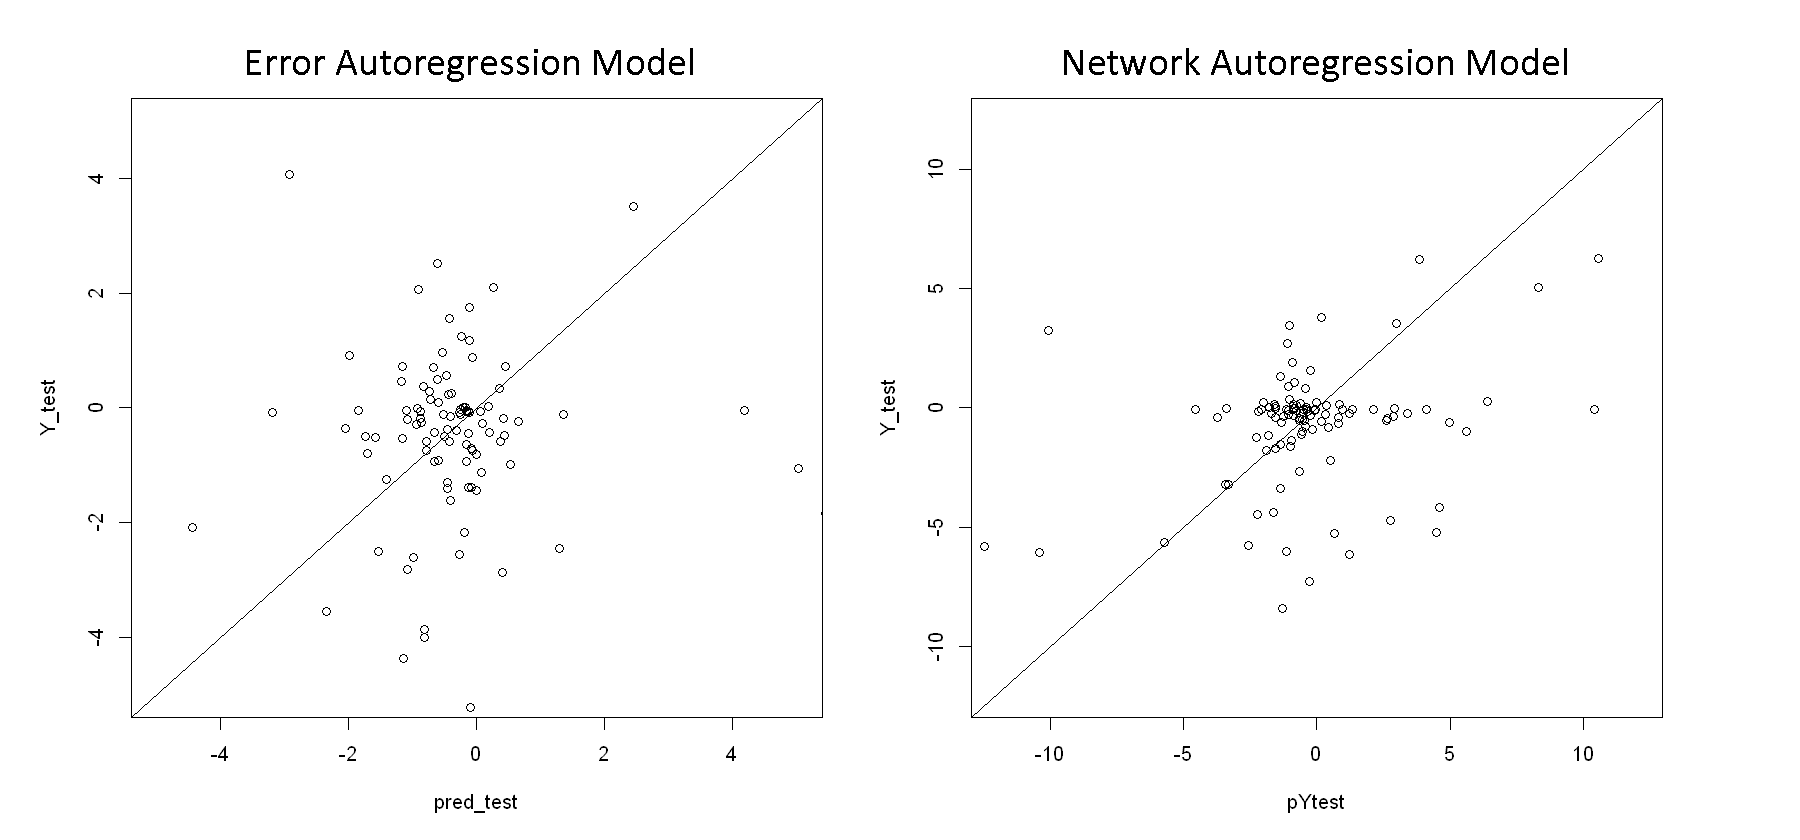
\includegraphics[width=\linewidth]{predictions.png}
	\caption{Actual vs Predicted changes in stock prices on the testing data}
	\label{fig: predicted_stocks}
\end{figure}


\section{Conclusion}
In this paper, we presented a multiple network regression framework which considered the autocorrelation that exist in the network data and interactions across multiple networks. The framework covered model selection, regression, estimation of autocorrelation and other model parameters, and model prediction. A new methodology for testing the significance of a network in a multiple network regression setting was developed. The test statistics were formulated based on the F-test statistic in multiple linear regression. Simulations confirmed that the two proposed tests, t-test and Moran's I normality test, can identify significant networks. Further, a Gibbs Sampler was developed to generate random numbers from the joint posterior distribution of the model parameters. A Method of predictions on the testing data was applied to generate the prediction distributions. The application of the proposed multiple network regression model on two real datasets indicated a good model accuracy in both cases.


%\references
%\begin{description}


\begin{thebibliography}{99}	
	
	
\bibitem[Advani \& Malde, 2018] {R31}
\textsc{Advani, ~A., \& Malde, ~B.} (2018). Credibly identifying social effects: Accounting for network formation and measurement error. \textit{Journal of Economic Surveys}. DOI: 10.1111/joes.12256

\bibitem[Anselin, 2009]{R1}
\textsc{Anselin, ~L.} (2009). Spatial regression. In: \textit{The SAGE handbook of spatial analysis}, \textbf{1}, 255-276.

\bibitem[Barabási, 2013]{R30}
\textsc{Barabási, ~A. ~L.} (2013). Network Science. \textit{Philosophical Transactions of the Royal Society A}, \textbf{371: 20120375}. DOI: 10.1098/rsta.2012.0375

\bibitem[Bivand{,} Gómez-Rubio \& Rue, 2014] {R37}
\textsc{Bivand, ~R. ~S., Gómez-Rubio, ~V., \& Rue, ~H.} (2014). Approximate Bayesian inference for spatial econometrics models, \textit{Spatial Statistics}, \textbf{9}, 146-165.

\bibitem[Bivand \& Wong, 2018]{R20}
\textsc{Bivand, ~R., \& Wong, ~D.} (2018). Comparing implementations of global and local indicators. \textit{TEST}, \textbf{27(3)}, 716-748.

\bibitem[Block{,} Hoffman{,} Raabe et al., 2020]{R27}
\textsc{Block, ~P., Hoffman, ~M., Raabe, ~I. ~J., Dowd, ~J. ~B., Rahal, ~C., Kashyap, ~R., \& Mills, ~M. ~C.} (2020). Social network-based distancing strategies to flatten the COVID-19 curve in a post-lockdown world. \textit{Nature Human Behaviour}, \textbf{4}, 588-596. DOI: 10.1038/s41562-020-0898-6

\bibitem[Bramoull\'e{,} Djebbari \& Fortin, 2009]{R2} 
\textsc{Bramoull\'e, ~Y., Djebbari, ~H., \& Fortin, B.} (2009). Identification of peer effects through social networks. \textit{Journal of Econometrics}, \textbf{150(1)}, 41-55.

\bibitem[Brasington \& Hite, 2005]{R3}
\textsc{Brasington, ~D., \& Hite, ~D.} (2005). Demand for Environmental Quality A Spatial Hedonic Analysis. \textit{Regional Science and Urban Economics}, \textbf{35(1)}, 57-82.

\bibitem[Elhorst \& Fr\'eret, 2009]{R4}
\textsc{Elhorst, ~J., \& Fr\'eret, ~S.} (2009). Evidence of Political Yardstick Compeition in France using a Two-Regime Spatial Durbin Model with Fixed effects. \textit{Journal of Regional Science}, \textbf{49(5)}, 931-951.

\bibitem[Elhorst, 2010]{R5}
\textsc{Elhorst, ~J.} (2010). Applied Spatial Econometrics: Rising the Bar. \textit{Spatial Economic Analysis}, \textbf{5(1)}, 9-28.

\bibitem[Elhorst, 2014]{R6}
\textsc{Elhorst, ~J.} (2014). Spatial Econometrics: From Cross-Sectional Data to Spatial Panels. Springer, Belin.

\bibitem[Elhorst{,} Lacombe \& Piras, 2012]{R42}
\textsc{Elhorst, ~J., Lacombe, ~D. ~J., \& Piras, ~G.} (2012). On model specification and parameter space definitions in higher order spatial econometric models. \textit{Regional Science and Urban Economics}, \textbf{42}, 211-220. DOI: 10.1016/j.regsciurbeco.2011.09.003

\bibitem[Fischer \& LeSage, 2014] {R32}
\textsc{Fischer, ~M.M., \& LeSage, ~J. ~P.} (2014). Spatial regression-based model specifications for exogenous and endogenous spatial interaction. \textit{ERSA conference papers}, \textbf{ersa14p716}, European Regional Science.

\bibitem[Florax \& Nijkamp, 2005] {R38}
\textsc{Florax, ~R., \& Nijkamp, ~P.} (2005). Misspecification in Linear Spatial Regression Models, \textit{Encyclopedia of Scoial Measurement}, 695-707.

\bibitem[Godoy-Lorite \& Jones, 2021]{R23}
\textsc{Godoy-Lorite, ~A., \& Jones, ~N.} (2021). Inference and influence of network structure using snapshot social behavior without network data. \textit{Science Advances}, \textbf{7(23)}, eabb8762, DOI: 10.1126/sciadv.abb8762

\bibitem[Heijmans \& Magnus, 1986]{R7} 
\textsc{Heijmans, ~R., \& Magnus, ~J.} (1986). Consistent maximum-likelihood estimation with dependent observations: the general (non-normal) case and the normal case. \textit{Journal of Econometrics}, \textbf{32(2)}, 253-285.

\bibitem[Kelejian \& Prucha, 2001]{R8}
\textsc{Kelejian, ~H., \& Prucha, ~I.} (2001). On the asymptotic distribution of the Moran I test statistic with applications. \textit{Journal of Econometrics}, \textbf{104(2)}, 219-257.

\bibitem[Kelejian \& Prucha, 2010]{R40}
\textsc{Kelejian, ~H., \& Prucha, ~I.} (2010). Specification and estimation of spatial autoregressive models with autoregressive and heteroskedastic disturbances. \textit{Journal of Econometrics}, \textbf{157(1)}, 53-67.

\bibitem[Kim \& Leskovec, 2012]{R22}
\textsc{Kim, ~M., \& Leskovec, ~J.} (2012). Multipicative Attribute Graph Model of Real World Networks. \textit{Internet Mathematics}, \textbf{8(1-2)}, 113-160, DOI: 10.1080/15427951.2012.625257

\bibitem[Kostov, 2009]{R9}
\textsc{Kostov, ~P.} (2009). A spatial quantile regression hedonic model of agricultural land prices. \textit{Spatial Economic Analysis}, \textbf{4(1)}, 53-72.

\bibitem[Lee, 2002]{R10} 
\textsc{Lee, ~L.} (2002). Consistency and Efficiency of Least Squares Estimation for Mixed Regressive, Spatial Autoregressive Models. \textit{Econometric Theory}, \textbf{18}, 252-277.

\bibitem[Lee, 2004]{R11} 
\textsc{Lee, ~L.} (2004). Asymptotic Distributions of Quasi-Maximum Likelihood Estimators for Spatial Autoregressive Models. \textit{Econometrica}, \textbf{72(6)}, 1899-1925.

\bibitem[Lee \& Ogburn, 2020] {R41}
\textsc{Lee, ~Y., \& Ogburn, ~E. ~L.} (2020). Testing for Network and Spatial Autocorrelation, In: Masuda N., Goh KI., Jia T., Yamanoi J., Sayama H. (eds) \textit{Proceedings of NetSci-X 2020: Sixth International Winter School and Conference on Network Science}, 91-104. Springer Proceedings in Complexity. Springer. DOI: 10.1007/978-3-030-38965-9-7. 

\bibitem[LeSage \& Pace, 2008] {R34}
\textsc{LeSage, ~J. ~P., \& Pace, ~R. ~K.} (2008). Spatial Econometric Modeling of Origin-Destination Flows, \textit{Journal of Regional Science}, \textbf{48(5)}, 941-967. DOI: 10.1111/j.1467-9787.2008.00573.x

\bibitem[LeSage, 2014]{R21}
\textsc{LeSage, ~J. ~P.} (2014).
What regional scientists need to know about spatial econometrics,
\textit{The Review of Regional Studies}, Southern Regional Science Association, vol. 44(1), 13-32.

\bibitem[Li{,} Hong{,} Tang et al., 2016] {R35}
\textsc{Li, ~L., Hong, ~X., Tang, ~D., \& Na, ~M.} (2016). GHG Emissions, Economic Growth and Urbanization: A Spatial Approach, \textit{Sustainability}, \textbf{8}, 462. DOI: 10.3390/su8050462

\bibitem[Manski, 1993]{R12}
\textsc{Manski, ~C.} (1993). Identification of Endogenous Social Effects: The Reflection Problem. \textit{The review of economic studies}, 60(3), 531-542.

\bibitem[Manski, 2000]{R13}
\textsc{Manski, ~C.} (2000). Economic Analysis of Social Interactions. \textit{Journal of Economic Perspectives}, \textbf{14(3)}, 115-136.

\bibitem[Nakagawa{,} Johnson{,} \& Schielzeth, 2017] {R39}
\textsc{Nakagawa, ~S., Johnson, ~P. ~C. ~D., Schielzeth, ~H.} (2017). The coefficient of determination R2 and intra-class correlation coefficient from generalized linear mixed-effects models revisited and expanded, \textit{Journal of the Royal Society Interface}, \textbf{14}, 20170213.

\bibitem[Newman{,} Barabási \& Watts, 2006]{R25}
\textsc{Newman, ~M., Barabási, ~A. ~L., \& Watts, ~D. ~J.} (2006). The Structure and Dynamics of Networks. \textit{Princeton University Press}.

\bibitem[Ogburn, 2018] {R33}
\textsc{Ogburn, ~E.L.} (2018). Challenges to estimating contagion effects from observational data. \textit{Complex Spreading Phenomena in Social Systems}, 47-64, Springer.

\bibitem[Pace \& LeSage, 2010] {R36}
\textsc{Pace, ~R. ~K., \& LeSage, ~J. ~P.} (2010). Omitted Variable Biases of OLS and Spatial Lag Models, In A.Páez, J.Gallo, R. N. Buliung, \& S. Dall'erba (Eds), \textit{Progress in Spatial Analysis}, 17-28, Berlin and Heidelberg. Springer.

\bibitem[Pan{,} McCormick \& Fosdick, 2021]{R24}
\textsc{Pan, ~M., McCormick, ~T., \& Fosdick, ~B.} (2021). Inference for Network Regression Models with Community Structure. \textit{arXiv:2106.04271v1}, DOI: arxiv.org/abs/2106.04271

\bibitem[Robinson, 2010]{R16} 
\textsc{Robinson, ~P.} (2010). Efficient estimation of the semiparametric spatial autoregressive model. \textit{Journal of Econometrics}, \textbf{157(1)}, 6-17.

\bibitem[Sampson{,} Morenoff \& Gannon-Rowley, 2002]{R17} 
\textsc{Sampson, ~R., Morenoff, ~J., \& Gannon-Rowley, ~T.} (2002). Assessing 'neighborhood effects': Social processes and new directions in research. \textit{Annual review of sociology}, \textbf{28(1)}, 443-478.

\bibitem[Takagi \& Shimada, 2019]{R28}
\textsc{Takagi, ~D., \& Shimada, ~T.} (2019). A Spatial Regression Analysis on the Effect of Neighborhood-Level Trust on Cooperative Behaviors: Comparison With a Multilevel Regression Analysis. \textit{Frontiers in Psychology}, \textbf{10}. DOI: 10.3389/fpsyg.2019.02799

\bibitem[Teng{,} Xu{,} Sandel et al., 2018]{R29}
\textsc{Teng, ~S.N., Xu, ~C., Sandel, ~B., \& Svenning, ~J.} (2018). Effects of intrinsic sources of spatial autocorrelation on spatial regression modeling. \textit{Methods in Ecology and Evolution}, \textbf{9}, 363-372. DOI: 10.1111/2041-210X.12866

\bibitem[Yu{,} Bai \& Ding, 2015]{R18} 
\textsc{Yu, ~D., Bai, ~P., \& Ding, ~C.} (2015). Adjusted quasi-maximum likelihood estimator for mixed regressive, spatial autoregressive model and its small sample bias. \textit{Computational Statistics and Data Analysis}, \textbf{87}, 116-135.

\bibitem[Zhang{,} Pan{,} Guan et al., 2020]{R26}
\textsc{Zhang, ~X., Pan, ~R., Guan, ~G., Zhu, ~X., \& Wang, ~H.} (2020). Logistic Regression with Network Structure. \textit{Statistica Sinica}, \textbf{30}, 673-693, DOI: 10.5705/ss.202017.0281

\bibitem[Zhou{,} Tu{,} Chen et al., 2017]{R19}
\textsc{Zhou, ~J., Tu, ~Y., Chen, ~Y., \& Want, ~H.} (2017). Estimating spatial autocorrelation with sampled network data. \textit{Journal of Business \& Economic Statistics}, \textbf{35(1)}, 130-138.

\end{thebibliography}
\end{document}

	
	